% This is paper draft
% edited by Haoruo Peng
% Date: 2013.9.5
\documentclass[10pt, conference, compsocconf]{IEEEtran}
\usepackage{amsmath, amssymb}
\usepackage{color}
\usepackage{graphicx}
\usepackage{bbding}
\usepackage{epstopdf}

\newcommand{\bw}{\mathbf{w}}
\newcommand{\bwep}{\mathbf{w}^{\varepsilon}}
\newcommand{\bwfly}{\tilde{\mathbf{w}}}
\newcommand{\bwavg}{\mathbf{wavg}}
\newcommand{\bu}{\mathbf{u}}
\newcommand{\buprev}{\mathbf{uprev}}
\newcommand{\bp}{\mathbf{p}}
\newcommand{\bq}{\mathbf{q}}
\newcommand{\bxi}{\mathbf{\xi}}
\newcommand{\dotwxb}{{\mathbf{w}}^{\mathbf{T}}\mathbf{x}_{i}+b}
\newcommand{\sumt}{\sum_{t=1}^{T} }
\newcommand{\lc}{\left(}
\newcommand{\rc}{\right)}
\newcommand{\li}{\lc i\rc}
\newcommand{\lj}{\lc j\rc}
\newcommand{\tspace}{\hspace*{2em}}
\newcommand{\tspaces}{\hspace*{1.5em}}
\newcommand{\comment}{\textcolor{red}}
\newcommand{\ti}[1]{\tilde{#1}}
\newcommand{\indep}{{\;\bot\!\!\!\!\!\!\bot\;}}

\def\A{{\bf A}}
\def\a{{\bf a}}
\def\B{{\bf B}}
\def\C{{\bf C}}
\def\c{{\bf c}}
\def\D{{\bf D}}
\def\d{{\bf d}}
\def\E{{\bf E}}
\def\e{{\bf e}}
\def\f{{\bf f}}
\def\K{{\bf K}}
\def\H{{\bf H}}
\def\G{{\bf G}}
\def\I{{\bf I}}
\def\R{{\bf R}}
\def\X{{\bf X}}
\def\Y{{\bf Y}}
\def\Q{{\bf Q}}
\def\s{{\bf s}}
\def\S{{\bf S}}
\def\x{{\bf x}}
\def\y{{\bf y}}
\def\z{{\bf z}}
\def\Z{{\bf Z}}
\def\M{{\bf M}}
\def\m{{\bf m}}
\def\n{{\bf n}}
\def\U{{\bf U}}
\def\u{{\bf u}}
\def\V{{\bf V}}
\def\v{{\bf v}}
\def\W{{\bf W}}
\def\w{{\bf w}}
\def\0{{\bf 0}}
\def\1{{\bf 1}}

\def\AM{{\mathcal A}}
\def\FM{{\mathcal F}}
\def\TM{{\mathcal T}}
\def\UM{{\mathcal U}}
\def\XM{{\mathcal X}}
\def\YM{{\mathcal Y}}
\def\NM{{\mathcal N}}
\def\OM{{\mathcal O}}
\def\IM{{\mathcal I}}
\def\GM{{\mathcal G}}
\def\RB{{\mathbb R}}

\def\tx{\tilde{\bf x}}
\def\ty{\tilde{\bf y}}
\def\tz{\tilde{\bf z}}
\def\hd{\hat{d}}
\def\HD{\hat{\bf D}}
\def\hx{\hat{\bf x}}

\def\alp{\mbox{\boldmath$\alpha$\unboldmath}}
\def\bet{\mbox{\boldmath$\beta$\unboldmath}}
\def\epsi{\mbox{\boldmath$\epsilon$\unboldmath}}
\def\etab{\mbox{\boldmath$\eta$\unboldmath}}
\def\ph{\mbox{\boldmath$\phi$\unboldmath}}
\def\pii{\mbox{\boldmath$\pi$\unboldmath}}
\def\Ph{\mbox{\boldmath$\Phi$\unboldmath}}
\def\Ps{\mbox{\boldmath$\Psi$\unboldmath}}
\def\tha{\mbox{\boldmath$\theta$\unboldmath}}
\def\Tha{\mbox{\boldmath$\Theta$\unboldmath}}
\def\muu{\mbox{\boldmath$\mu$\unboldmath}}
\def\Si{\mbox{\boldmath$\Sigma$\unboldmath}}
\def\Gam{\mbox{\boldmath$\Gamma$\unboldmath}}
\def\Lam{\mbox{\boldmath$\Lambda$\unboldmath}}
\def\De{\mbox{\boldmath$\Delta$\unboldmath}}
\def\vps{\mbox{\boldmath$\varepsilon$\unboldmath}}

\def\Ncal{\mathcal{N}}
\def\argmax{\mathop{\rm argmax}}
\def\argmin{\mathop{\rm argmin}}

\def\sgn{\mathrm{sgn}}
\def\tr{\mathrm{tr}}
\def\rk{\mathrm{rank}}
\def\diag{\mathsf{diag}}
\def\vect{\mathsf{vec}}
\def\etal{{\em et al.\/}\,}

\begin{document}

\title{Evaluating Parallel Logistic Regression Models}

\author{
\IEEEauthorblockN{Haoruo Peng}
\IEEEauthorblockA{HTC Research Center\\Beijing, China\\penghaoruo@hotmail.com}
\and
\IEEEauthorblockN{Ding Liang}
\IEEEauthorblockA{HTC Research Center\\Beijing, China\\Ding\_Liang@htc.com}
\and
%\IEEEauthorblockN{Deli Zhao}
%\IEEEauthorblockA{HTC Research Lab\\Beijing, China\\zhaodeli@gmail.com}
%\and
\IEEEauthorblockN{Cyrus Choi}
\IEEEauthorblockA{HTC Research Center\\Beijing, China\\Cyrus\_Choi@htc.com}
}

\maketitle

\begin{abstract}
Logistic regression (LR)  has been widely used in applications of machine learning, thanks to its linear model.
However, when the size of training data is very large, even such a linear model can consume excessive memory and computation time.  To tackle both resource and computation scalability in a big-data setting, we evaluate and compare different approaches in distributed platform, parallel algorithm, and sublinear approximation.  Our empirical study provides design guidelines for choosing the most effective combination for the performance requirement of a given application.
\end{abstract}

\begin{IEEEkeywords}
Logistic Regression Model; Parallel Computing; Sublinear Method; Big Data;
\end{IEEEkeywords}

\section{Introduction} \label{sec:int}
The logistic regression model~\cite{HastieBook:SL} plays a pivotal role in machine learning tasks.
%It is a widely used model in applications such as PageRank~\cite{page1999pagerank} and anti-spam %filtering~\cite{androutsopoulos2000evaluation}.
The model is suited for classification problems and is supported by a substantial body of statistical theories.
A binary classification problem modeled by LR can be easily extended to a multi-class classification problem.
We focus our study on the binary LR model in this paper (and the conclusions can be extended to a multi-class setting).

In recent years, many modern datasets have grown drastically in both data volume and data dimensionality.
Large data volume and high data dimensionality bring both resource and computational challenges to machine learning algorithms.
For example, a social networking site such as Facebook consists of tens of millions of records, each is composed of hundreds of attributes. For text and multimedia categorization, we usually have to deal with billion-scale datasets in a feature space of thousands of dimensions.  In this work, we evaluate approaches to scale up LR in a big-data setting.  The approaches we evaluate include three aspects: 1) distributed platform, 2) parallel algorithm, and 3) sublinear approximation.

In the platform aspect, we compare two well known distributed systems:
 Hadoop~\cite{white2012hadoop} and Spark~\cite{zaharia2010spark}.
Hadoop employs HDFS~\cite{borthakur2008hdfs} and MapReduce~\cite{dean2008mapreduce}.
Spark promotes the efficiency of iterative algorithms and also supports HDFS.
In the parallel algorithm aspect, we compare the sequential optimization algorithms: stochastic gradient descent~\cite{zhang2004solving}, which can
obtain optimal generalization guarantees with a small number of passes over the data.
 The algorithm can easily be parallelized on either Hadoop or Spark, and it can also be used in an online setting, at which a data instance is seen only once in a streaming fashion.  Finally, to further speed up computation, we compare aforementioned platform/algorithm combinations with our previously proposed sublinear algorithms~\cite{peng2012sublinear}.
These sublinear algorithms access a single feature of a feature vector instead of all features at each iteration to reduce computation time.
Our evaluation and comparisons provide insights to facilitate an application designer for selecting a solution that best meets the performance requirement of the machine-learning task at hand.

\section{Related Work} \label{sec:rew}

%\subsection{Scalability Solutions}
%
%In big data scenarios, large datasets require us to develop machine learning algorithms towards a more efficient and more parallelized end. Researchers have already done much work to cater for the needs of massive datasets. Early work like Parallel Support Vector Machines (PSVM)~\cite{chang2011psvm} employed an approximation matrix decomposition method based on row selections to reduce memory usage. It can then increase the number of parallel computational nodes to several hundreds. Later, the work of Parallel Latent Dirichlet Allocation (PLDA)~\cite{Liu:2011:PPL:1961189.1961198}~\cite{newman2007distributed} improves the computational efficiency of the LDA model by means of sampling methods. The parallel algorithm in Hadoop is robust, for it has fault tolerance of machine failures, thus taking advantage of Hadoop features. Recently, Dean \etal~\cite{le2011building} claimed that the advantage of parallelization is fully taken in deep learning algorithms. It pushed the limit of parallel computational nodes to a hundred-million level, and in the meantime, achieved the best learning performance ever. GraphLab~\cite{kyrola2012graphchi} is a recently developed tool for large-scale machine learning. It tackles efficiency and scalability problems of machine leaning algorithms by graph-theoretical models.

We present related work in the two aspects: platform and algorithm.
\subsection{Computing Platforms}\label{sec:platform}
The two distributed platforms that we work with have their
own advantages in the implementation of machine learning algorithms.
The Hadoop~\cite{white2012hadoop} platform allows for distributed processing of large datasets across clusters of computers using simple programming models. It utilizes MapReduce~\cite{dean2008mapreduce} as its computational paradigm, which is easily parallelized. Additionally, Hadoop provides a Distributed File System (HDFS). Both MapReduce and HDFS are designed to handle node failures in an automatic way, allowing Hadoop to support large clusters that are built on commodity hardware.
Spark~\cite{zaharia2010spark} is a cluster computing system that aims to make data analysis fast. It supports the in-memory cluster computing. A job can load data into memory and query it repeatedly by creating and caching resilient distributed datasets (RDDs). Moreover, RDDs achieve fault tolerance through lineage: information about how RDDs are derived from other RDDs is stored in reliable storage, thus making RDDs easy to be rebuilt if a certain partition is lost. Spark can execute up to be two orders faster than Hadoop for iterative algorithms.

Table~\ref{tab:systemcmp} compares different features between Hadoop and Spark platforms.
Spark supports two types of operations on RDDs: Actions and Transformations (As and Ts).
Actions include functions like \textit{count}, \textit{collect} and \textit{save}. They usually return a result from input RDDs.
Transformations include functions like \textit{map}, \textit{filter} and \textit{join}. They normally build new RDDs from other RDDs, which comply with the lineage rule.
In the table, we use ``NFS" to denote ``Normal File System".\

\begin{table}[h]
\centering
\caption{Platform Comparison: Hadoop vs. Spark}\label{tab:systemcmp}\vspace{-0.3cm}
\begin{tabular}{|c|c|c|}
\hline
           & Hadoop & Spark \\
\hline
Computational Paradigm  & MapReduce & As and Ts \\
\hline
File System Supported & HDFS & HDFS and NFS \\
\hline
Design Concept  & Key-value Pairs & RDD \\
\hline
Fault Tolerance Technique & Redundancy & Lineage \\
\hline
\end{tabular}
%\vspace{-0.5cm}
\end{table}

It is worth mentioning that Apache Mahout~\cite{mahoutscalable} runs on Hadoop and is a scalable machine learning library. Mahout integrates many important algorithms for clustering, classification and collaborative filtering in its package. It is highly optimized so that Mahout also achieves good performance for non-distributed algorithms. We use Mahout as the baseline in our experiments.

\subsection{Sublinear Methods}

Sublinear methods have recently been proposed by several researchers.
Clarkson \etal~\cite{clarkson2010sublinear} first presented the solution of approximation algorithms in sublinear time.
The algorithm employs a novel sampling technique along with a new multiplicative update procedure.
Hazan \etal~\cite{hazanbeating} exploited the approach to speed up linear SVMs.
Cotter \etal~\cite{cotter2012kernelized} extended the method to kernelized SVMs.
In~\cite{hazan2011optimal}, Hazan \etal applied the sublinear approximation approach to solve linear regression with penalties.
Garber and Hazan~\cite{garberapproximating} also developed sublinear method with Semi-Definite Programming (SDP).
Peng \etal~\cite{peng2012sublinear} utilized the method in the LR model with penalties and developed sequential sublinear algorithms for both $\ell_1$-penalty and $\ell_2$-penalty.

\subsection{Other Related Work}

LR is fairly straightforward to be parallelized.   Parallelization efforts on several machine learning algorithms such as SVMs~\cite{chang2011psvm}, LDA~\cite{Liu:2011:PPL:1961189.1961198}, Spectral Clustering~\cite{Chen5444877}, and frequent itemset mining~\cite{Li:2008:PPF:1454008.1454027} require much more sophisticated sharding work to divide a computational task evenly onto distributed subtasks.  For a comprehensive survey, please consult~\cite{chang2011foundations} and~\cite{Bekkerman2012}.

\section{Logistic Regression Model and Sequential Sublinear Algorithm} \label{sec:plr}

\subsection{Logistic Regression Model} \label{sec:def}
In this paper, we mainly concern the binary classification problem.  	
We define the training dataset as $\XM=\{(\x_i, y_i): i=1, \ldots, n\}$, where $\x_i \in \RB^d$ are input samples and $y_i \in \{-1, 1\}$ are the corresponding labels.
For simplicity, we will use the notation $\X=[{\x}_{1}, {\x}_{2}, \ldots, {\x}_n]^{T}$ and $\y=(y_1, y_2, \ldots, y_n)^T$ to represent the training dataset in this paper.
To fit in the logistic regression model, the expected value of $y_i$ is given by\vspace{-0.2cm}
\[
P(y_i|\x_i)= \frac{1}{1+ \exp(- y_i(\x_i^T \w + b))} \triangleq g_i(y_i),\vspace{-0.2cm}
\]
where $\w=(w_1, \ldots, w_d)^T \in \RB^d$ is a regression vector and $b\in \RB$ is an offset term.

The learning process aims to derive $\w$ and $b$ by solving an optimization problem.
It is a common practice to add penalties to LR model in order to avoid overfitting and make the optimization result more practical.
Typically, for $\ell_2$-penalty, we solve the following optimization problem:\vspace{-0.2cm}
\begin{equation} \label{eqn:1}
	\max_{\bw ,b} \; \Big\{F(\w, b| \XM) - \frac{\lambda}{2}  \|\bw\|_2^{2} \Big\}.\vspace{-0.2cm}
\end{equation}
For $\ell_1$-penalty, we optimize the following criterion: \vspace{-0.2cm}
\begin{equation} \label{eqn:2}
	\max_{\bw ,b} \;  \big\{F(\w, b|\XM)- \gamma{\|\bw \|}_{1}\big\}.\vspace{-0.2cm}	
\end{equation}
Here, we define $F(\w, b| \XM) = \sum_{i=1}^n \log g_i(y_i)$ in both (\ref{eqn:1}) and (\ref{eqn:2}). To be brief, we omit the derivation here.

\subsection{Sequential Sublinear Algorithm}
We use the following notations to define sequential sublinear algorithm for penalized logistic regression. Function $clip\lc \cdot \rc$ is a projection function defined as $
clip\lc a,b \rc \triangleq \max \lc \min \lc a,b \rc ,-b\rc,\,a,b\in \mathbb{R}$.
Function $\sgn \lc \cdot \rc$ is the sign function; namely, $\sgn \lc \cdot \rc \in \{-1,0,1\}$.
$g\lc \cdot \rc$ is the logistic function $g \lc x \rc=1/(1+e^{-x})$.

In Algorithm~1, we give the sequential sublinear approximation procedure for logistic regression. The algorithm is from our previous work~\cite{peng2012sublinear}. Mathematical symbols we use here comply with definitions in Section~\ref{sec:def}. Parameter $\varepsilon$ controls learning rate, $T$ determines iteration number, and $\eta$ defines approximation level. Details of the parameter initialization step are documented in~\cite{peng2012sublinear}.

	\begin{table} [ht]
	\begin{tabular}{l}
	\hline\noalign{\smallskip}
	\textbf{Algorithm 1}: Sub-Linear Logistic Regression (SLLR) \\
	\noalign{\smallskip}
	\hline
	\noalign{\smallskip}
	1:	Input parameters: $\varepsilon, \nu~or~\gamma, X, Y$ \\
	2:	Initialize parameters: $T, \eta, {\mathbf{u}}_{0}, {\bw}_{1}, {\mathbf{\bq}}_{1}, {b}_{1}$\\
	3:	Iterations: $t=1 \sim T$ \\
	4:	\tspace ${\bp}_{t}\leftarrow{\bq}_{t}/{\|{\bq}_{t}\|}_{1}$ \\
	5:  \tspace Choose ${i}_{t}\leftarrow i$ with probability $\bp(i)$ \\
	6:	\tspace $coef\leftarrow{y}_{{i}_{t}}g\lc-{y}_{{i}_{t}}\lc {{\bw}_{t}}^{T}{\mathbf{x}}_{i_t}+{b}_{t} \rc\rc$ \\
	7:	\tspace ${\bu}_{t}\leftarrow {\bu}_{t-1}+\frac{coef}{\sqrt{2T}}{\mathbf{x}}_{{i}_{t}}$ \\
    8:  \tspace ${\bxi}_{t}\leftarrow \argmax_{\bxi\in \Lambda}\lc{{\bp}_{t}}^{T}\bxi\rc$, if input $\nu$ for $\ell_2$-penalty \\
    9:  \tspace $\bu_t\leftarrow$ soft-thresholding operations, if input $\gamma$ for $\ell_1$-penalty \\
	10:	\tspaces ${\bw}_{t}\leftarrow {\bu}_{t}/\max \left\{1,\|{\bu}_{t}\|_2 \right\}$ \\
    11: \tspaces ${b}_{t}\leftarrow \sgn\lc {{\bp}_{t}}^{T}\mathbf{y}\rc$ \\
	12:	\tspaces Choose ${j}_{t}\leftarrow j$ with probability ${{\bw}_{t}\lj}^{2}/{\|{\bw}_{t}\|_2}^{2} $ \\
	13:	\tspaces Iterations: $i=1 \sim n$ \\
	14:	\tspaces\tspace $\sigma \leftarrow \mathbf{x}_{i} \lc {j}_{t}\rc{\|{\bw}_{t}\|_2}^{2}/{\bw}_{t}\lc {j}_{t} \rc+{\bxi}_{t}\li+{y}_{i}{b}_{t}$ \\
	15:	\tspaces\tspace $\hat{\sigma} \leftarrow clip\lc \sigma,1/\eta \rc$ \\
	16:	\tspaces\tspace ${\bq}_{t+1}\li \leftarrow {\bp}_{t}\li\lc 1-\eta\hat{\sigma} + {\eta}^{2}{\hat{\sigma}}^{2} \rc$ \\
	17:	Output: $\bar{\bw}=\frac{1}{T}\sum_{t}{\bw}_{t},\bar{b}=\frac{1}{T}\sum_{t}{b}_{t}$ \\
	\hline
	\end{tabular} 	
	\label{alg:1}
	\end{table}

Each iteration of the SLLR algorithm has two phases: \textit{stochastic primal update} and \textit{stochastic dual update}.
Steps from line $4$ to line $11$ consist of the primal part while the dual part is composed of steps from line $12$ to line $16$.
We give the sublinear algorithm in a unified way for $\ell_2$-penalty and $\ell_1$-penalty.
If we are dealing with $\ell_2$-penalty, we ignore line 9 and accomplish the computation in line 8 by a simple greedy algorithm.
Here, $\Lambda$ represents a Euclidean space with conditions $
\Lambda=\left\{ \bxi\in\mathbb{R}_{n} \, | \, \forall i, \, 0\leq{\xi}_{i}\leq 2, \, {\|\xi \|}_{1}\leq \nu n  \right
\}$.
If we are faced with $\ell_1$-penalty, we ignore line $8$ and expand the procedure of line $9$ as the following:

\begin{table} [ht]
\begin{tabular}{l}
\hline\noalign{\smallskip}
\textbf{Procedure}: Line 9 in Algorithm 1\\
\noalign{\smallskip}
\hline
\noalign{\smallskip}
Iterations: $j=1 \sim d$ \\
\tspace \textbf{if} $\buprev_t\lj>0$ \textbf{and} $\bu_t\lj>0$ \\
\tspace\tspace $\bu_t\lj=\max \lc \bu_t\lj-\gamma ,0 \rc$ \\
\tspace \textbf{if} $\buprev_t\lj<0$ \textbf{and} $\bu_t\lj<0$ \\
\tspace\tspace $\bu_t\lj=\min \lc \bu_t\lj+\gamma ,0 \rc$ \\
$\buprev_{t+1}\leftarrow\bu_t$ \\
\hline
\end{tabular}
\end{table}

In this sequential mode, each iteration takes $O(n+d)$ time, which is sublinear to the dataset size.

\section{Parallel Sublinear Logistic Regression} \label{sec:framework}
In this section, we describe our parallel sublinear algorithms implemented on Hadoop and Spark, respectively.
We also formally introduce the traditional parallel gradient algorithm used in Spark and the online stochastic gradient descent method used in Mahout.
In all pseudo-code, we follow symbol notations defined in Section~\ref{sec:def}.
\subsection{Parallel Sublinear Algorithms on Hadoop}
We develop an algorithm to achieve sublinear performance for learning logistic regression parameters using the architecture of MapReduce.
The pseudo-code of Algorithm 2, together with auxiliary procedures, explains the critical parts of this algorithm.

	\begin{table}[ht]
	\begin{tabular}{l}
	\hline\noalign{\smallskip}
	\textbf{Algorithm 2}: PSUBPLR-MR \\
	\noalign{\smallskip}
	\hline
	\noalign{\smallskip}
    1:  Input parameters: $\varepsilon, \nu~or~\gamma, X, Y, n, d$ \\
    2:	Initialize parameters: $T, \eta, {\mathbf{u}}_{0}, {\bw}_{1}, {\mathbf{\bq}}_{1}, {b}_{1}$\\
    3:	Iterations: $t=1 \sim T$ \\
    4:  \tspace $\bw_t \rightarrow$ storeInHdfsFile("hdfs://paraw").addToDistributedCache() \\
    5:  \tspace $\bp_t \rightarrow$ storeInHdfsFile("hdfs://parap").addToDistributedCache() \\
    6:  \tspace conf\_primal $\leftarrow$ new Configuration() \\
    7:  \tspace job\_primal $\leftarrow$ new MapReduce-Job(conf\_primal) \\
    8:  \tspace conf\_primal.passParameters($T, n, d, b_t$) \\
    9:  \tspace job\_primal.setInputPath("...") \\
	10:	\tspaces job\_primal.setOutputPath("tmp/primal$t$") \\
    11: \tspaces job\_primal.run() \\
    12: \tspaces ($\bw_{t+1}, b_{t+1}$)$\leftarrow$Primal-Update($\bw_t, b_t$) \\
    13: \tspaces Choose $j_t \leftarrow j$ with probability ${{\bw}_{t+1}\lj}^{2}/{\|{\bw}_{t+1}\|_2}^{2} $ \\
    14: \tspaces $\bw_{t+1} \rightarrow$ storeInHdfsFile("hdfs://paraw").addToDistributedCache() \\
    15: \tspaces conf\_dual $\leftarrow$ new Configuration() \\
    16: \tspaces job\_dual $\leftarrow$ new MapReduce-Job(conf\_dual) \\
    17: \tspaces conf\_dual.passParameters($d, j_t, b_{t+1}, \eta$) \\
    18: \tspaces job\_primal.setInputPath("...") \\	
    19:	\tspaces job\_dual.setOutputPath("tmp/dual$t$") \\
    20: \tspaces job\_dual.run() \\	
    21: \tspaces $\bp_{t+1}\leftarrow$Dual-Update($\bp_t$) \\
    22: Output: $\bar{\bw}=\frac{1}{T}\sum_{t}{\bw}_{t},\bar{b}=\frac{1}{T}\sum_{t}{b}_{t}$ \\
	\hline
	\end{tabular}
	\end{table}
     %
    \begin{table}[ht]
	\begin{tabular}{l}
	\hline\noalign{\smallskip}
	\textbf{Procedure}: Primal-Map(inputfile) \\
	\noalign{\smallskip}
	\hline
	\noalign{\smallskip}
    1:  ~Configuration.getParameters($T, n, d, b_t$) \\
    2:  ~$\bw_t \leftarrow$ readCachedHdfsFile("paraw") \\
    3:  ~$\bp_t \leftarrow$ readCachedHdfsFile("parap") \\
    4:  ~$i_t \leftarrow$ parseRowIndx(inputfile)\\
    5:  ~$\mathbf{x}_{i_t} \leftarrow$ parseRowVector(inputfile) \\
    6:  ~$y_{i_t} \leftarrow$ parseRowLabel(inputfile) \\
    7:  ~$r \leftarrow$ \textit{random(seed)} \\
    8:  ~\textbf{if} $\bp_t(i_t) > \frac{r}{n}$ \\
    9:  ~\tspace $tmp\_coef=\bp_t(i_t){y}_{{i}_{t}}g\lc-{y}_{{i}_{t}}\lc {{\bw}_{t}}^{T}{\mathbf{x}}_{i_t}+{b}_{t} \rc\rc$ \\
    10: \textbf{else} \\
    11: \tspace $tmp\_coef=0$ \\
    12: Iterations: $j=1 \sim d$ \\
    13: \tspace Set $key \leftarrow j$ \\
    14: \tspace Set $value \leftarrow \frac{tmp\_coef}{\sqrt{2T}}\mathbf{x}_{i_t}(j) $ \\
    15: \tspace \textbf{Output}(key, value) \\
	\hline
	\end{tabular}
	\end{table}
    %
    \begin{table}[ht]
	\begin{tabular}{l}
	\hline\noalign{\smallskip}
	\textbf{Procedure}: Primal-Reduce(key\_in, value\_in) \\
	\noalign{\smallskip}
	\hline
	\noalign{\smallskip}
    1:  $key\_out \leftarrow key\_in$ \\
    2:  $value\_out \leftarrow \sum_{for~same~key\_in}{value\_in} $ \\
    3:  \textbf{Output}(key\_out, value\_out) \\
	\hline
	\end{tabular}
	\end{table}
    %
    \begin{table}[ht]
	\begin{tabular}{l}
	\hline\noalign{\smallskip}
	\textbf{Procedure}: Primal-Update($\bw_t, b_t$) \\
	\noalign{\smallskip}
	\hline
	\noalign{\smallskip}
    1:  $\Delta \bw_t \leftarrow$ readFromHdfsFile("tmp/primal$t$") \\
    2:  $\bw_{t+1} \leftarrow \bw_t+\Delta \bw_t$ \\
	3:	${\bw}_{t+1}\leftarrow {\bw}_{t+1}/\max \left\{1,\|{\bw}_{t+1}\|_2 \right\}$ \\
    4:  ${b}_{t+1}\leftarrow \sgn\lc {{\bp}_{t}}^{T}\mathbf{y}\rc$ \\
	\hline
	\end{tabular}
	\end{table}
    %
    \begin{table}[ht]
	\begin{tabular}{l}
	\hline\noalign{\smallskip}
	\textbf{Procedure}: Dual-Map(inputfile) \\
	\noalign{\smallskip}
	\hline
	\noalign{\smallskip}
    1:  ~Configuration.getParameters($d, j_t, b_{t+1}, \eta$) \\
    2:  ~$\bw_{t+1} \leftarrow$ readCachedHdfsFile("paraw") \\
    3:  ~$i_t \leftarrow$ parseRowIndx(inputfile)\\
    4:  ~$\mathbf{x}_{i_t} \leftarrow$ parseRowVector(inputfile) \\
    5:  ~$y_{i_t} \leftarrow$ parseRowLabel(inputfile) \\
    6:  ~$\sigma \leftarrow \mathbf{x}_{i_t} \lc {j}_{t}\rc{\|{\bw}_{t+1}\|_2}^{2}/{\bw}_{t+1}\lc {j}_{t} \rc+{y}_{i_t}{b}_{t+1}$ \\
	7:	~$\hat{\sigma} \leftarrow clip\lc \sigma,1/\eta \rc$ \\
	8:	~$res \leftarrow 1-\eta\hat{\sigma} + {\eta}^{2}{\hat{\sigma}}^{2} $ \\
    9:  ~$key \leftarrow i_t$ \\
    10: $value \leftarrow res $ \\
    11: \textbf{Output}(key, value) \\
	\hline
	\end{tabular}
	\end{table}
    %
    \begin{table}[ht]
	\begin{tabular}{l}
	\hline\noalign{\smallskip}
	\textbf{Procedure}: Dual-Update($\bp_t$) \\
	\noalign{\smallskip}
	\hline
	\noalign{\smallskip}
    1:  $\mathbf{var} \leftarrow$ readFromHdfsFile("tmp/dual$t$") \\
    2:  Iterations: $j=1 \sim n$ \\
    3:  \tspace $\bp_{t+1}(j) \leftarrow \bp_t(j)*\mathbf{var}(j)$ \\
	\hline
	\end{tabular}
	\end{table}

This parallel design generally follows the framework of sequential sublinear algorithm.
It has two computational components in each iteration: the primal update part from lines $4$ to $12$ and the dual update part from lines $13$ to $21$.
In the primal update part, there is a parallel implementation segment from lines $4$ to $11$, and also an unavoidable sequential segment as on line $12$.
In the dual part, it is the same situation that steps from lines $14$ to 20 employ parallel implementation, whereas the sequential bottleneck is from lines $13$ to $21$.
As the primal part and the dual part do not exhibit any inter-dependency, they can be executed simultaneously in each computation iteration.  This halves the computation time.
This framework is shown in Fig.~\ref{fig:frame}.
%
\begin{figure}[tb]
\center 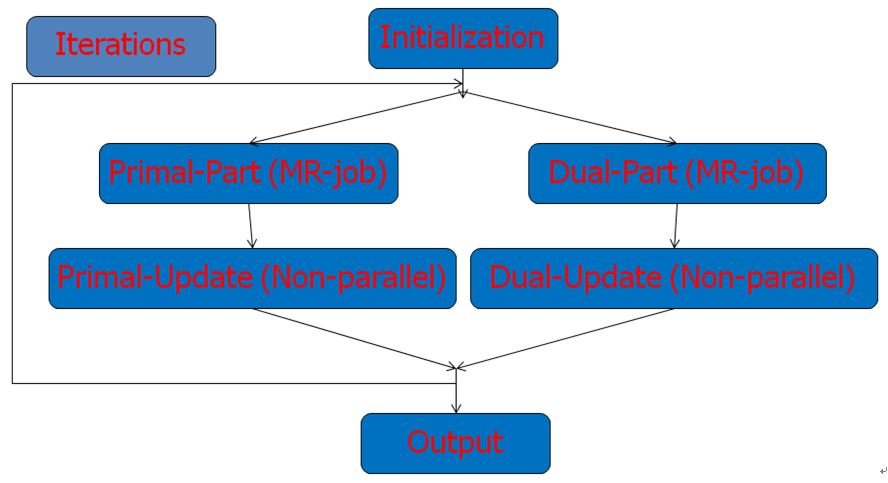
\includegraphics[height=3.0cm,width=6.5cm]{img/framework.png}\vspace{-0.3cm}
\caption{Parallel implementation flow chart for PSUBPLR-MR}\label{fig:frame}\vspace{-0.5cm}
\end{figure}
%

In the parallelization segment of the \textit{primal mapreduce job}, we process all data instances in parallel.
In the primal update step, we compute gradients from ``almost" all data instances and make the weighted average value according to vector $\bp$ as the output gradient for update.
The details of this algorithm design is shown in Procedure Primal-Map and Procedure Primal-Reduce.
Here, we employ a randomization strategy when we compute those ``almost" all gradients.
From lines $7$ to $8$ in Procedure Primal-Map, all data instances are computed if $r=0$.
As the expectation value for $\bp_t(i_t)$ is $\frac{1}{n}$, we normally set $r$ to range between zero to one.

Two more issues must be taken care of by the algorithm.
The first issue is parameter passing. It is critical to choose an efficient way to pass the updated parameters between iterations and even between different MapReduce jobs. The design of Hadoop requires passing parameters between computation iterations through files.  This IO step between iterations is clearly a bottleneck.

%The second issue is the small changes that we make to cater for the $\ell_2$-penalty and $\ell_1$-penalty. %The changes are only made in Procedure Primal-Update. It affects little for the implementation, and the %extension is just the same as that in Algorithm~1. To make the framework brief and standard, we omit the %explanation here.

The second issue is that datasets are generally sparse when the data dimension is high. This characteristic makes us focus on dealing with data sparsity issue in our code. Instead of naively writing the simple code in data intensive situations, we only store pairs of \textit{index} and \textit{value} in a data vector.
This sparse format brings us great memory-use efficiency improvement.

\subsection{Parallel Sublinear algorithms on Spark}
The algorithm to solve sublinear learning for penalized logistic regression in Spark is shown below.
In the pseudo-code of Algorithm 3, the procedure for Primal-Update and the procedure for Dual-Map are the same as those in Algorithm PSUBPLR-MR.
    \begin{table}[ht]
	\begin{tabular}{l}
    \hline\noalign{\smallskip}
	\textbf{Algorithm 3}: PSUBPLR-SPARK \\
	\noalign{\smallskip}
	\hline
	\noalign{\smallskip}
    1:  ~Input parameters: $\varepsilon, \nu~or~\gamma, X, Y, n, d$ \\
    2:	~Initialize parameters: $T, \eta, {\mathbf{u}}_{0}, {\bw}_{1}, {\mathbf{\bq}}_{1}, {b}_{1}$\\
    3:  ~points $\leftarrow$ spark.textFile(inputfile).map(parsePoint()).cache() \\
    4:  ~Iterations: $t=1 \sim T$ \\
    5:  ~\tspace gradient $\leftarrow$ points.map($(\frac{1}{1+e^{-y((\bw_t^T \textbf{x})+b)}}-1) * y * \bp [index]$) \\
        ~~~\tspace\tspace\tspace\tspace\tspace .reduce(sum()) \\
    6:  ~\tspace ($\bw_{t+1}, b_{t+1}$)$\leftarrow$Primal-Update($\bw_t, b_t$) \\
    7:  ~\tspace Choose $j_t \leftarrow j$ with probability ${{\bw}_{t+1}\lj}^{2}/{\|{\bw}_{t+1}\|_2}^{2} $ \\
    8:  ~\tspace pAdjust $\leftarrow$ points.map(MW-Update()).reduce(copy()) \\
    9:  ~\tspace $\bp_{t+1}\leftarrow$Dual-Update($\bp_t$)  \\
    10: \textbf{Output}($\bw, b$) \\
    \hline
    \end{tabular}
	\end{table}

This parallel design is very similar to that of Algorithm PSUBPLR-MR.
The most important difference is the \textit{cache()} operation in line 3.
To make it work in Spark, we follow the rule to construct an RDD for each data instance.
Also to cater for data sparsity, the design is that every data \textit{value} correspond to its individual \textit{index}. And the \textit{index} is also involved in the computation along with the \textit{value}.
We omit the changes for $\ell_2$-penalty and $\ell_1$-penalty here to make the algorithm easier to be understood.

In parallel mode, the primal update contains the update of $\bw_t$, which takes $O(n)$ time.
The dual update contains the $\ell_2$-sampling process for the choice of $j_t$ in $O(d)$ time, and the update of $\bp$ in $O(1)$ time.
Altogether, each iteration takes $O(n+d)$ time.
Compared to the analysis of sequential algorithm, parallelization does not necessarily change computational complexity.
Theoretically, parallel sublinear algorithm can be two times faster than the sequential version as the time for both update procedures in each iteration is reduced to $O(1)$.
Moreover, by starting two separate MapReduce jobs in one iteration simultaneously, the running time can be reduced to $O(max\{n,d\})$.

\subsection{Parallel Gradient Descent in Spark}
The parallel gradient descent method to solve LR in Spark is shown below.
    \begin{table}[ht]
	\begin{tabular}{l}
    \hline\noalign{\smallskip}
	\textbf{Algorithm 4}: PGDPLR-SPARK \\
	\noalign{\smallskip}
	\hline
	\noalign{\smallskip}
    1:  Input parameters: $\varepsilon, \nu~or~\gamma, X, Y, n, d$ \\
    2:	Initialize parameters: $T, \eta, {\mathbf{u}}_{0}, {\bw}_{1}, {\mathbf{\bq}}_{1}, {b}_{1}$\\
    3:  points $\leftarrow$ spark.textFile(inputfile).map(parsePoint()).cache() \\
    4:  Iterations: $t=1 \sim T$ \\
    5:  \tspace gradient $\leftarrow$ points.map($(\frac{1}{1+e^{-y((\bw_t^T \textbf{x})+b)}}-1)*y$) \\
        ~~\tspace\tspace\tspace\tspace\tspace .reduce(sum()) \\
    6:  \tspace $\bw_{t+1} = \bw_t - gradient * \textbf{x}$ \\
    7:  \tspace $b = b - gradient$ \\
    8:  \textbf{Output}($\bw, b$) \\
    \hline
    \end{tabular}
	\end{table}

The pseudo-code of Algorithm 4 shows that the algorithm is naturally parallelizable.
We can take in all data in the same iteration and just compute the gradient in a MapReduce fashion.
As for the \textit{cache()} operation and RDD design for data sparsity, it is the same with Algorithm PSUBPLR-SPARK.

\subsection{Online Stochastic Gradient Descent in Mahout}
Though SGD is an inherently sequential algorithm, it is blazingly fast. Thus Mahout's implementation can handle training sets of tens of millions of instances.
The SGD system in Mahout is an online learning algorithm, implying that we can learn models in an incremental fashion instead of traditional batching.
In addition, we can halt training when a model reaches target performance.
Because the SGD algorithms need feature vectors of fixed length and it is very costly to build a dictionary ahead of time, most SGD applications use an encoding system to derive hashed feature vectors. We can create a \textit{RandomAccessSparseVector}, and then use various feature encoders to progressively add features to this vector.
In our implementation, we use \textit{RandomAccessSparseVector} for data sparsity and the function call by \textit{OnlineLogisticRegression} to train the LR classifier.
We also perform cross validation. However, to maintain consistency with other methods for a fair comparison, we write our own code to ensure the same cross validation scheme is applied to all algorithms being evaluated.
	
\section{Experimental Setup} \label{sec:setup}
This section presents the details of the dataset information and testing environment of our experiments.

\subsection{Dataset Information}
We choose five open datasets to run all six test programs. Details are shown in Table~\ref{tab:table1}.	
Different from the simulated \textbf{2d} dataset, the other four datasets are all sparse.
We split each dataset into the training set and the testing set. We randomly repeat such split 20 times and our analysis is based on the average performance of 20 repetitions. In Table~\ref{tab:table1}, \textit{Density} is computed as
\[
Density(Dataset)~=~\frac{\#~of~Nonzeros}{\#~of~all~entries},
\]
which stems from~\cite{sarwar2001item}.
\textit{Balance} describes the binary distribution of labels.
We compute it as following:
\[
Balance(Dataset)~=~\frac{\#~of~Positive~Instances}{\#~of~Negative~Instances}.
\]
\begin{table*}%[h]
\centering
\caption{Datasets}\label{tab:table1}\vspace{-0.3cm}
\begin{tabular}{|c|c|c|c|c|c|c|c|}
\hline
    Name           & Dimension & \# of instances & Density  & \# of nonzero values & Balance & \# of training & \# of testing\\
\hline
    2d             & 2             & 200            & 1.0                      & 400          & 1.000 & --- & --- \\
\hline
    20NewsGroup    & 16428         & 1988           & $7.384\times10^{-3}$     & 238511          & 1.006 & 1800 & 188\\
\hline
    Gisette        & 5000          & 7000           & 0.12998                  & 4549319          & 1.000 & 6000 & 1000\\
\hline
    ECUESpam       & 100249        & 10687          & $2.563\times10^{-3}$     & 2746159          & 5.882 & 9000 & 1687\\
\hline
    URL-Reputation & 3231961       & 2376130        & $3.608\times10^{-5}$     & 277058644          & 0.500 & 2356130 & 20000\\
\hline
\end{tabular}
%\vspace{-0.3cm}
\end{table*}
These five datasets are carefully selected with an incremental trend in size.
The simulated \textbf{2d} dataset represents toy data situations and serves for the initial test of correctness of classifiers.
The \textbf{20NewsGroup} dataset is best-known for the test of LR model, which has a balanced distribution between positive and negative data instances. It also shows the application towards topic classification.
The \textbf{Gisette} dataset~\cite{guyon2004result} is relatively larger, and feature vectors are less sparse.
The \textbf{ECUESpam} dataset~\cite{DelanyKBS05} is selected due to its imbalanced distribution between positive and negative data instances. It has a higher data dimensionality than the \textbf{Gisette} dataset. However, because of data sparsity, it has fewer nonzero values involved in the computation.
Finally, the \textbf{URL-Reputation} dataset~\cite{ma2009identifying} contains millions of data instances and features. The raw data are stored in the SVM-light format, which has the volume of more than 2GB. It can be seen as a representative of massive datasets in the sense that it exceeds the scalability of Liblinear, which will be shown below.

\subsection{Testing Environment}
There are all together 6 test programs for comparison.
Online stochastic gradient descent method is run on Mahout in the sequential mode.
Liblinear~\cite{fan2008liblinear} is also a baseline test program we choose. It is sequential and outperforms many other programs for LR on a single machine.
SLLR performs the sequential sublinear algorithm on a single machine.
PSUBPLR-MR performs the parallel sublinear algorithm on Hadoop.
PGDPLR-SPARK is the test program for the parallel gradient descent run on Spark.
PSUBPLR-SPARK implements the parallel sublinear algorithm run on Spark.

We run our test programs on a six-node cluster, confiured as shown in Table~\ref{tab:table2}.  This computing cluster is considered small in size.  Nevertheless, past works (documented in \cite{chang2011foundations} and~\cite{Bekkerman2012}) in parallelization show that this configuration suffices to tell the trend of scalability.  Our future work will use a  larger cluster to run on much larger scale datasets in production settings to validate our conjecture.

\begin{table}[h]
\centering
\caption{Cluster Information}\label{tab:table2}\vspace{-0.3cm}
\begin{tabular}{|c|c|}
\hline
    CPU Model & Intel Xeon E5-1410: 2.80GHz \\
\hline
    Number of node & 6 \\
\hline
    Number of CPU per node & 4 Cores, 8 Threads \\
\hline
    RAM per node & 16G \\
\hline
    Disk per node & 4T HDD\\
\hline
    Interconnection Method & Gigabyte Ethernet  \\
\hline
\end{tabular}
\end{table}


\section{Experimental Results} \label{sec:experiment}
This section conducts analysis on experimental results.
We report and analyze results in 1) accuracy, 2) efficiency, 3) scalability and 4) robustness.

\subsection{Results on Precision} \label{sec:precision}
The results of six test programs achieved on five datasets are shown in Table~\ref{tab:table3}.
%
\begin{table}[h]
\centering
\caption{Accuracy Results. The meanings of abbreviations are as follows: 20-N-G, 20 News Group; URL-R, URL-Reputation.}\label{tab:table3}\vspace{-0.3cm}
\begin{tabular}{|c|c|c|c|c|}
\hline
           & 20-N-G & Gisette & ECUESpam & URL-R \\
\hline
Mahout     & 71.3\% & 91.5\% & 85.2\% & 91.5\% \\
\hline
Liblinear  & \textbf{92.0\%} & \textbf{97.4\%} & \textbf{97.1\%} & --- \\
\hline
SLLR       & 91.5\% & 94.8\% & 92.3\% & 94.2\% \\
\hline
PSUBPLR-MR & 90.5\% & 94.6\ & 91.7\% & 93.8\% \\
\hline
PGDPLR-SPARK & \textbf{92.0\%} & 97.0\% & 93.7\% & \textbf{96.0\%} \\
\hline
PSUBPLR-SPARK & 90.5\% & 95.8\% & 91.7\% & 94.0\% \\
\hline
\end{tabular}
\end{table}
%
These are the average results of running cross validation. Note that Liblinear cannot be implemented with the full \textbf{URL-Reputation} dataset on our machines due to memory limitation.
In Figures~\ref{fig:accuracy} (a)-(d), we show the test error as a function of iteration number on each dataset for all six test programs.

%
\begin{figure*}[tb]
\begin{center}
\begin{tabular}{cccc}
   %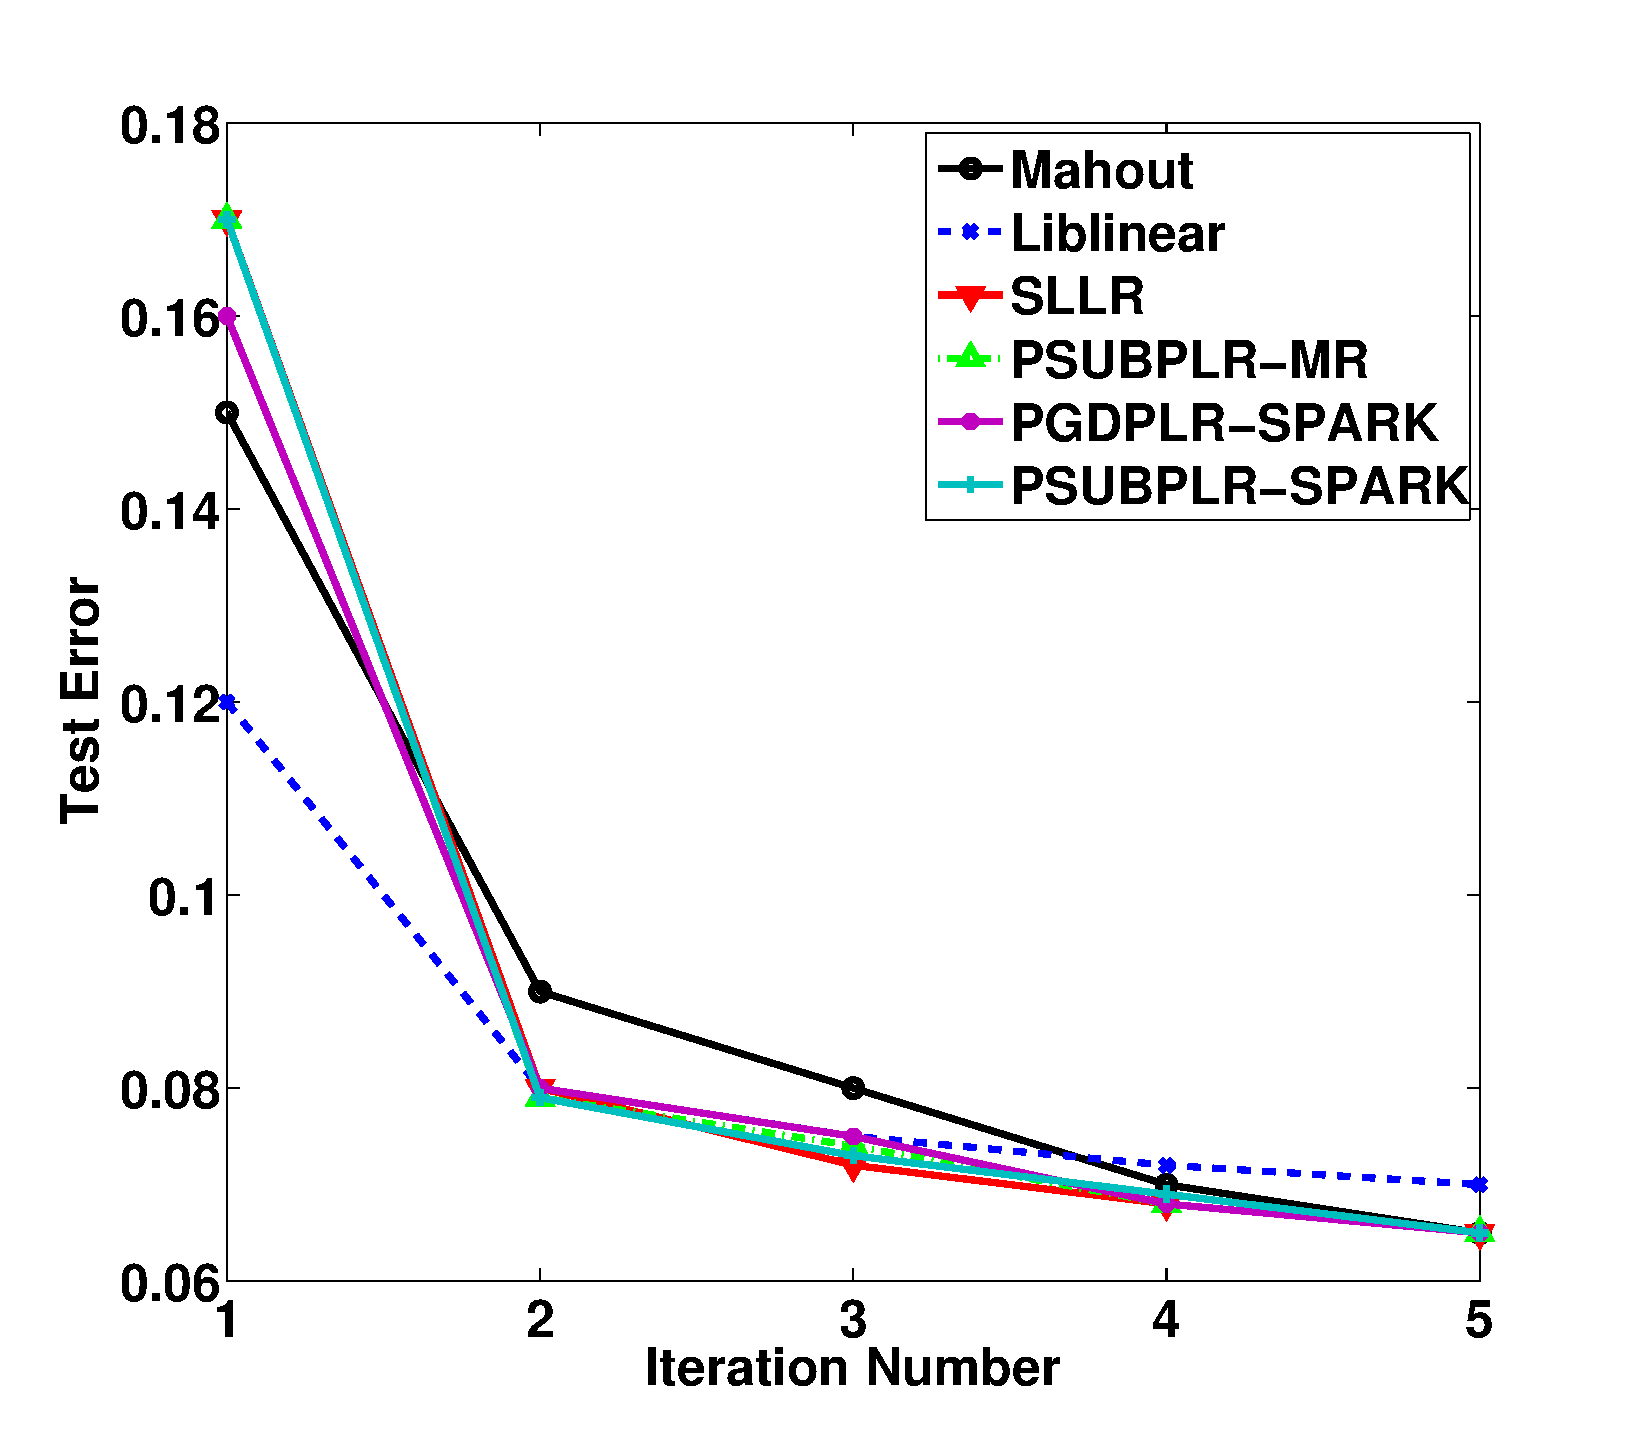
\includegraphics[height=4.5cm,width=5cm]{img/2d_accuracy_iteration.eps}&
   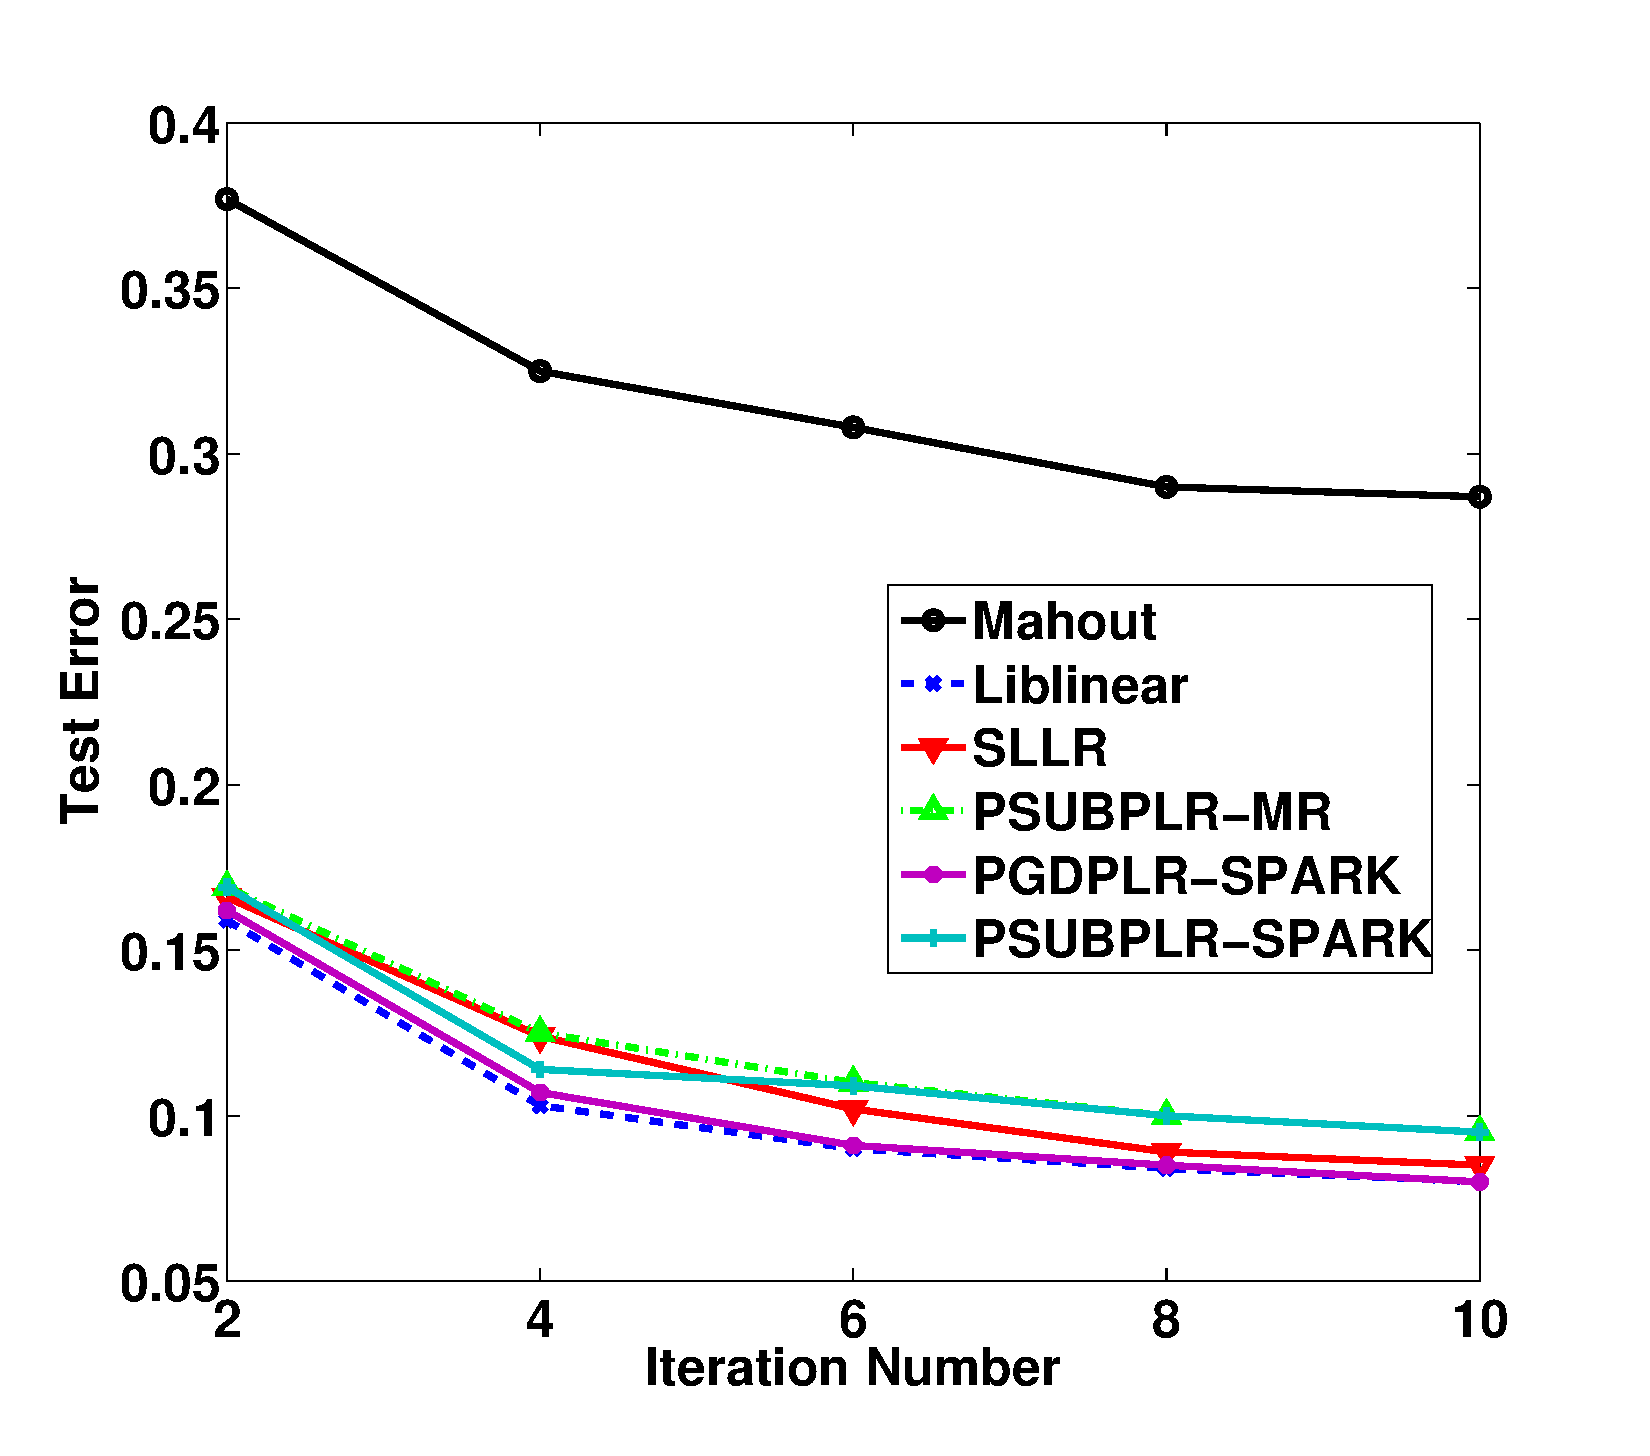
\includegraphics[height=4.cm,width=4.5cm]{img/20NewsGroup_accuracy_iteration.eps}&
   \hspace{-0.6cm}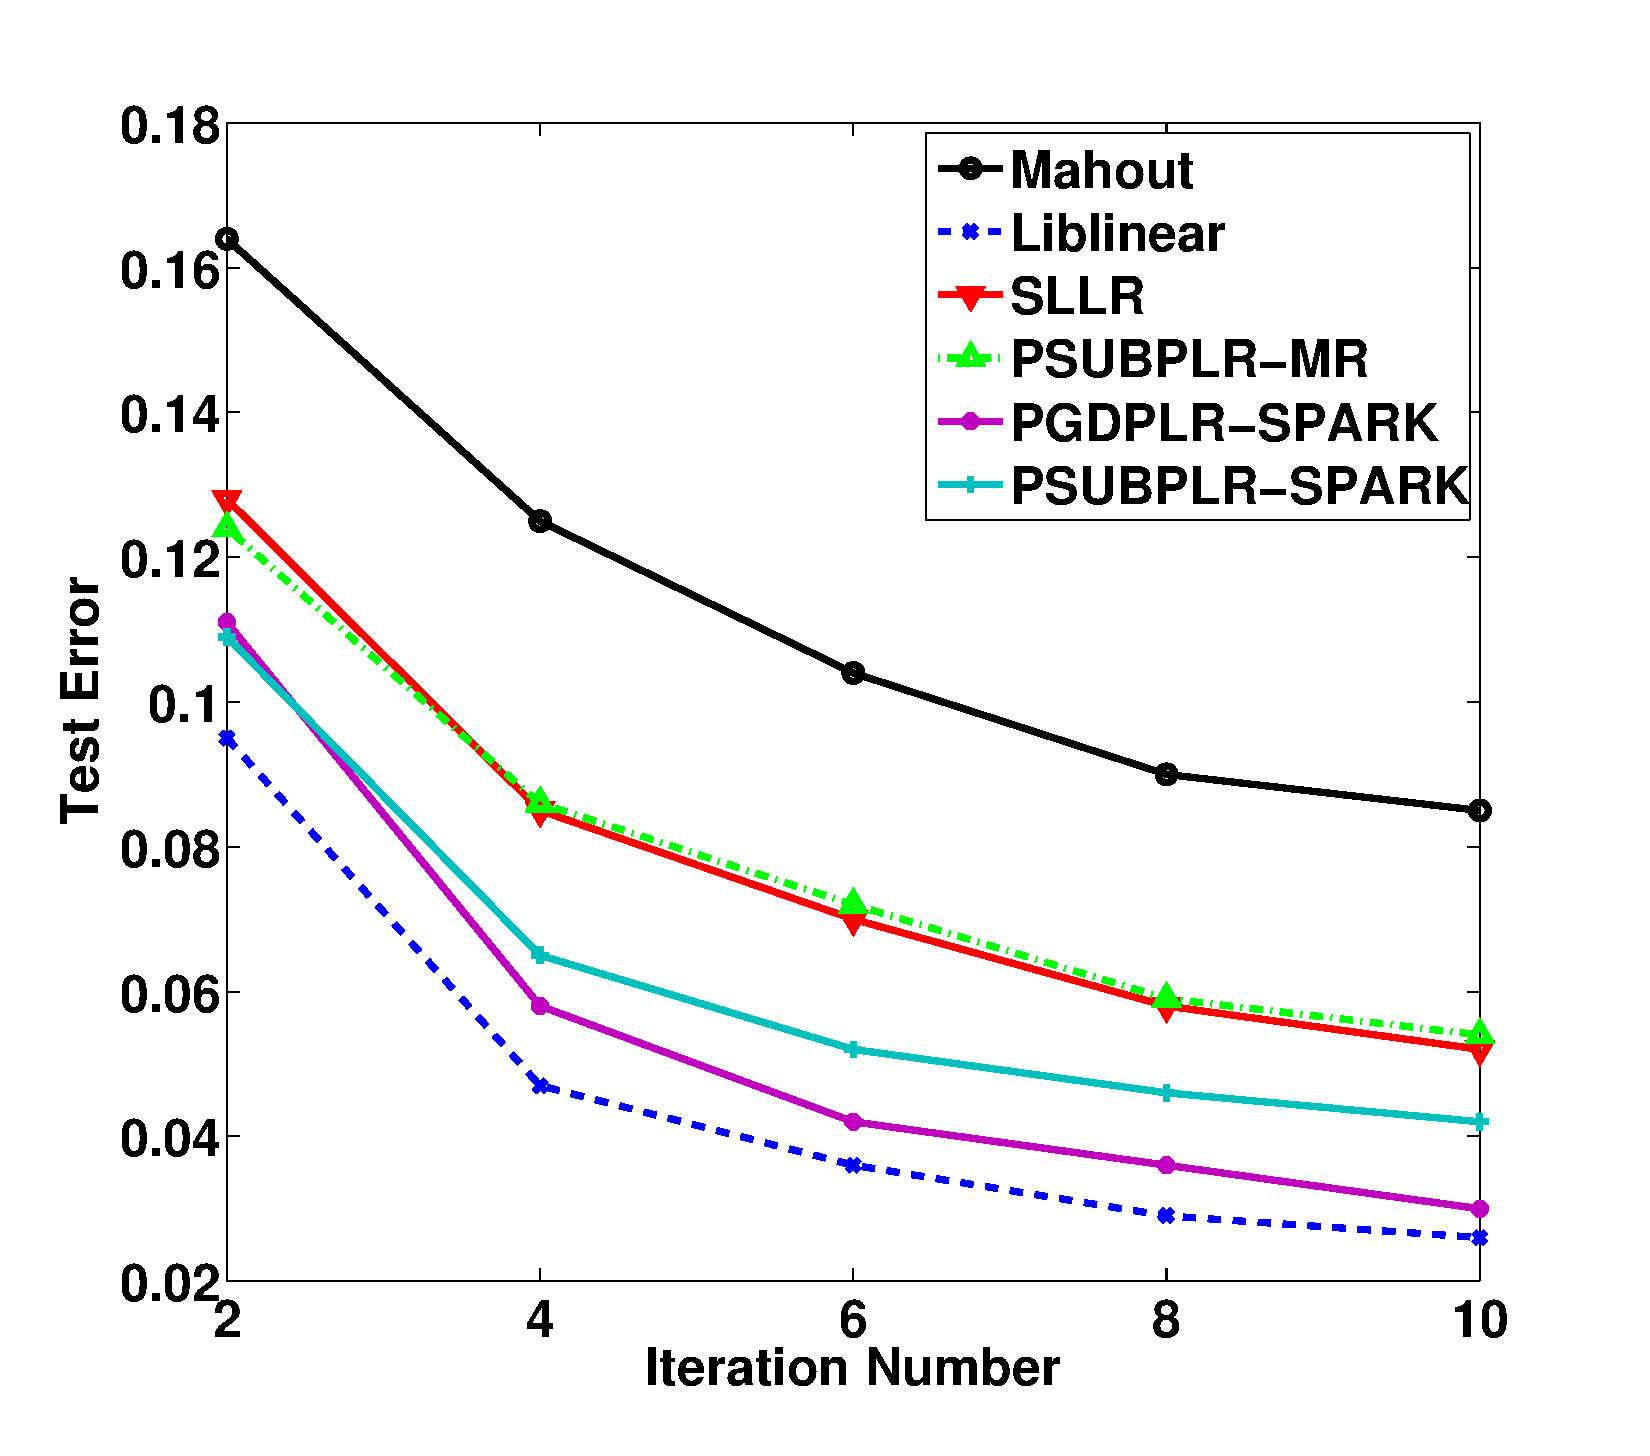
\includegraphics[height=4.cm,width=4.5cm]{img/Gisette_accuracy_iteration.eps}&
   \hspace{-0.6cm}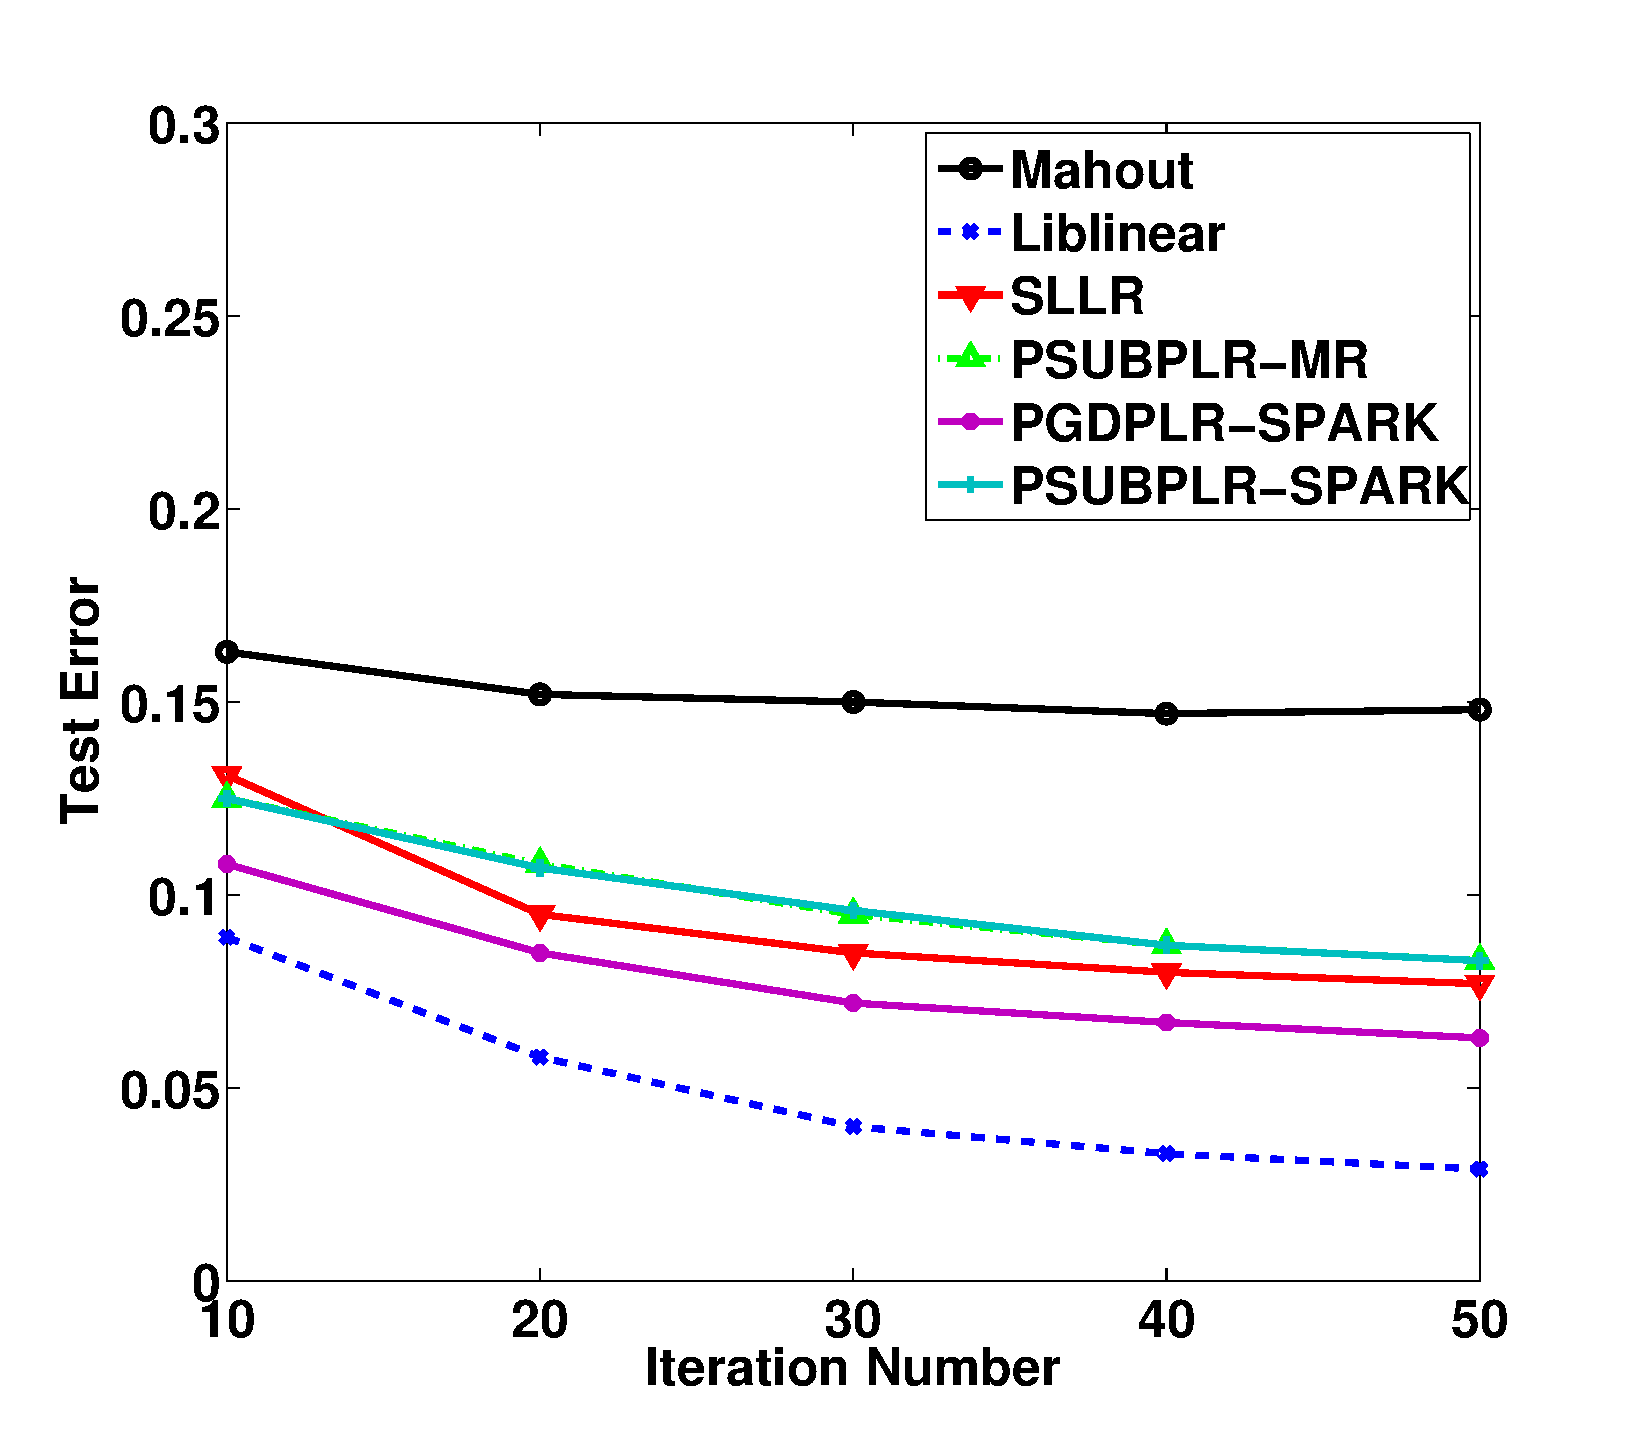
\includegraphics[height=4.cm,width=4.5cm]{img/ECUESpam_accuracy_iteration.eps}&
   \hspace{-0.6cm}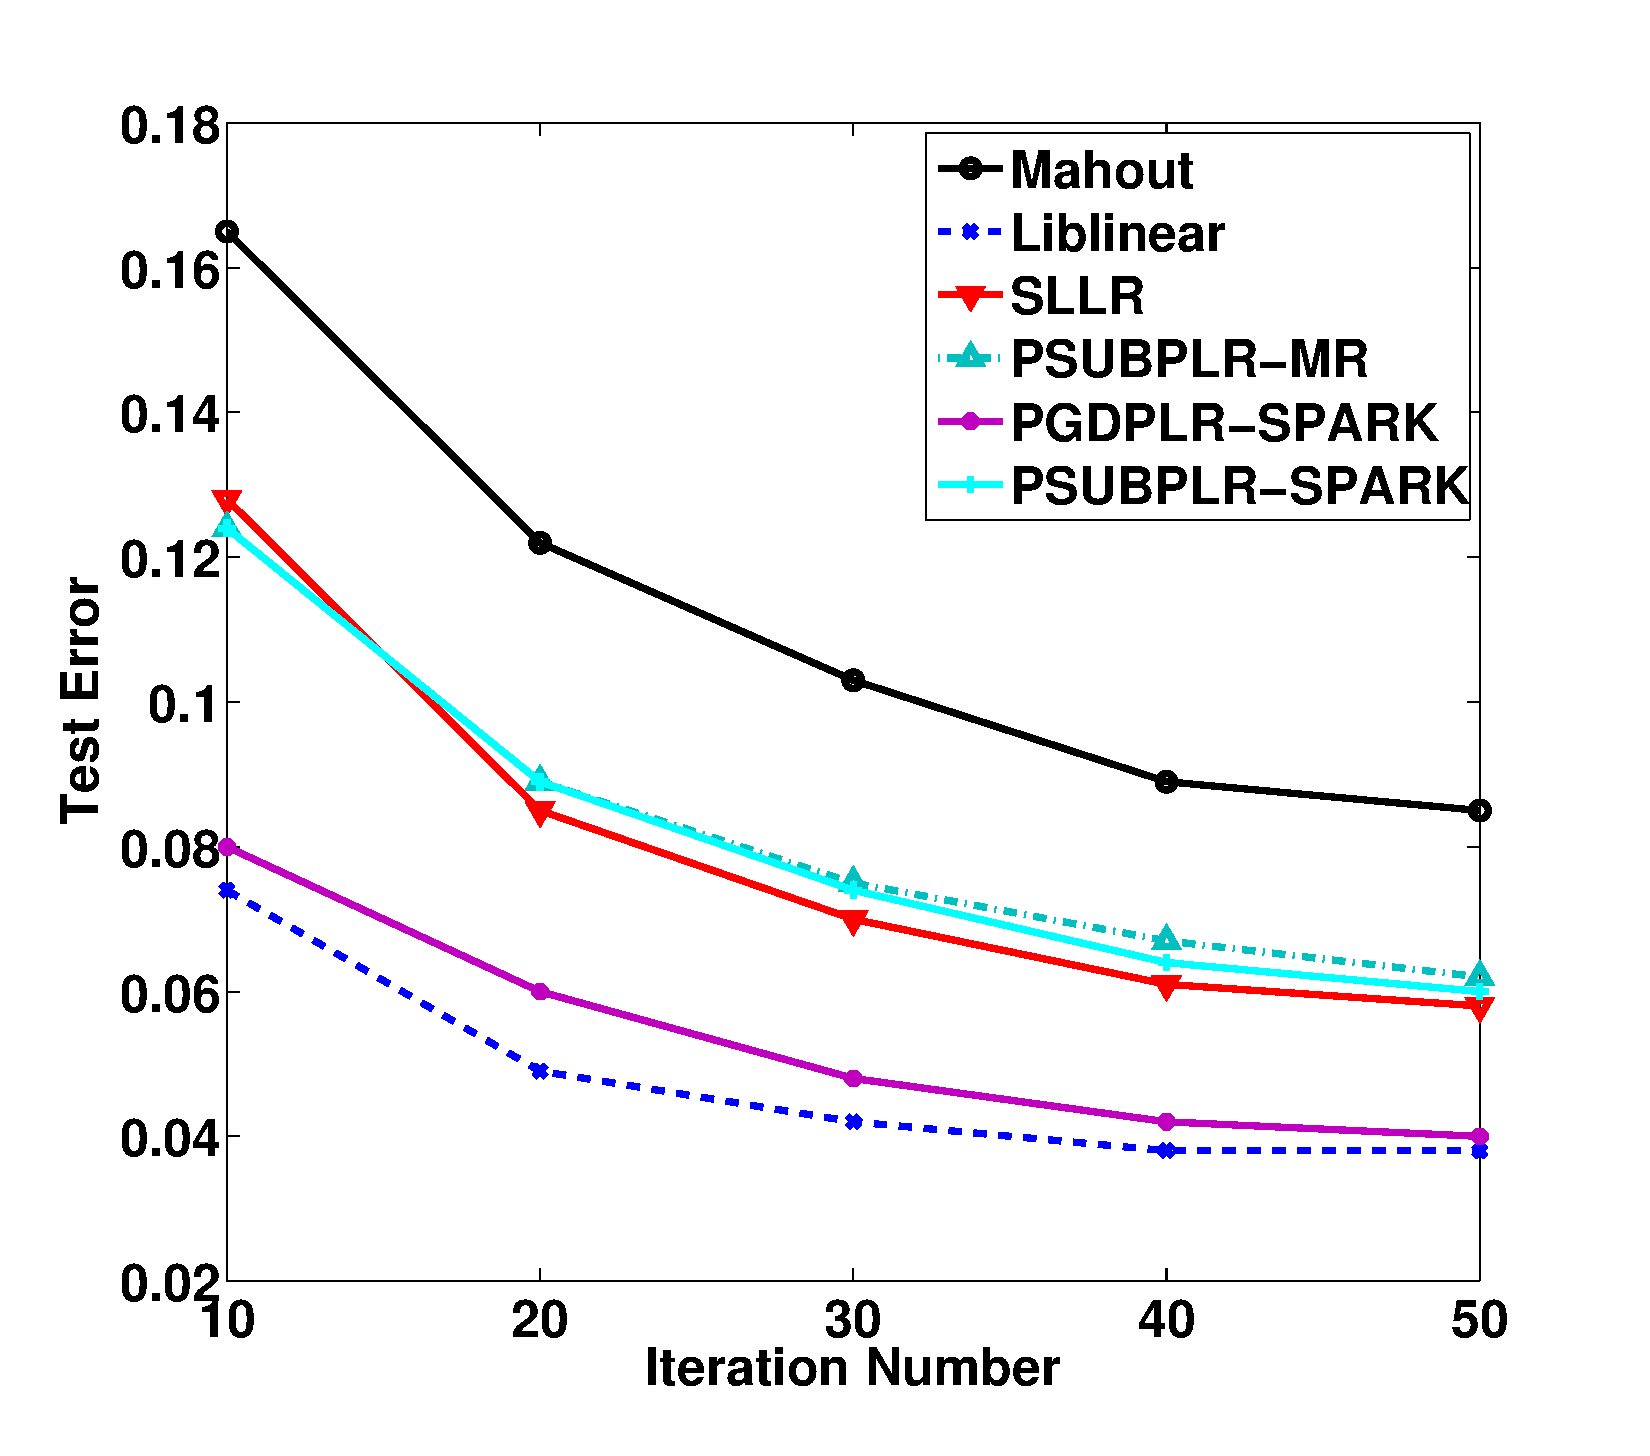
\includegraphics[height=4.cm,width=4.5cm]{img/URL-Reputation_accuracy_iteration.eps}\\
   (a) \textbf{20NewsGroup}. & \hspace{-0.3cm}(b) \textbf{Gisette}. & \hspace{-0.3cm}(c) \textbf{ECUESpam}. & \hspace{-0.3cm}(d) \textbf{URL-Reputation}.\\
   \end{tabular}
\end{center}
%\vspace{-0.3cm}
   \caption{Test error, as a function of iteration number.}\vspace{-0.5cm}
\label{fig:accuracy}
\end{figure*}

\subsection{Results on Running Time} \label{sec:time}

The running time of six test programs used on five datasets is shown in Table~\ref{tab:table4}.
The reported running time is the average of our corss-validation executions. Fig.~\ref{fig:08} reports the same results graphically.
%
\begin{table}[h]
\centering
\caption{Running Time. The meanings of abbreviations are as follows: 20-N-G, 20 News Group; URL-R, URL-Reputation.}\label{tab:table4}\vspace{-0.3cm}
\begin{tabular}{|c|c|c|c|c|c|}
\hline
           & 20-N-G & Gisette & ECUESpam & URL-R \\
\hline
Mahout     & 9.83s & 131.8s & 96s & 10100s \\
\hline
Liblinear  & \textbf{0.79s} & \textbf{2.4s} & \textbf{13s} & --- \\
\hline
SLLR       & 20.05s & 130.5s & 1028s & 3248s \\
\hline
PSUBPLR-MR & 1360.85s & 3687.9s & 11478s & 16098s \\
\hline
PGDPLR-SPARK & 10.52s & 99.2s & 924s & 3615s \\
\hline
PSUBPLR-SPARK & 8.57s & 89.1s & 796s & \textbf{2918s} \\
\hline
\end{tabular}
\end{table}


\begin{figure}[tb]
\center 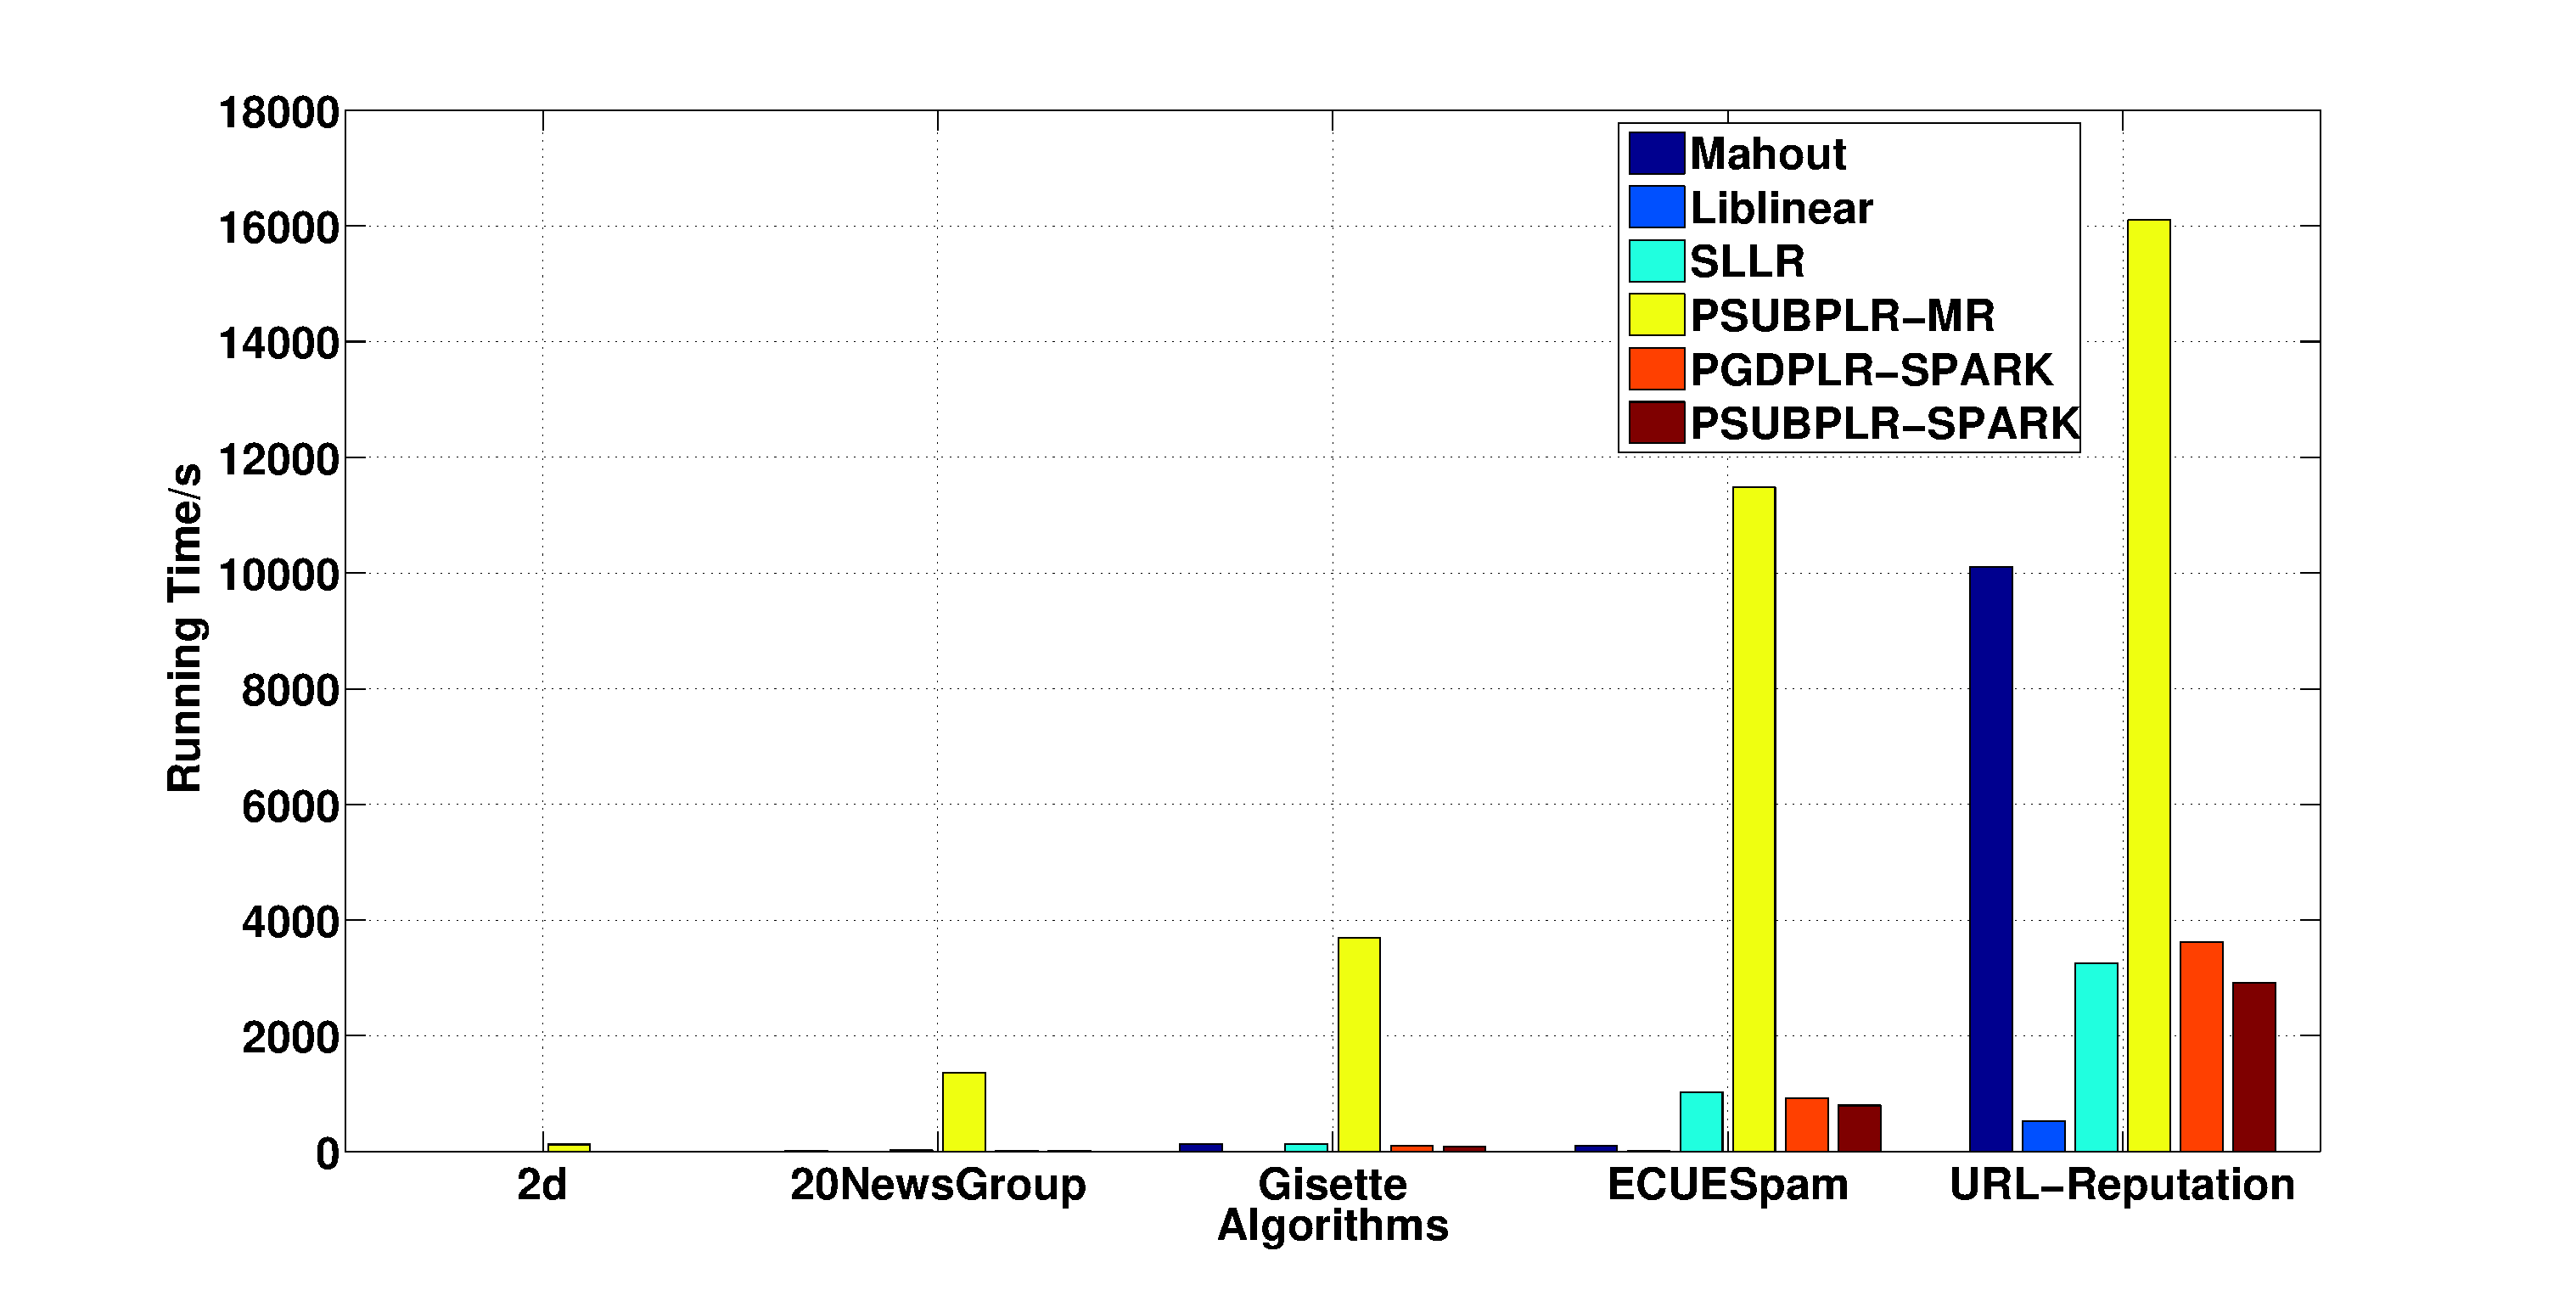
\includegraphics[height=4.8cm,width=9cm]{img/all_time.eps}
\vspace{-0.3cm}
\caption{Running time.}\label{fig:08}
\vspace{-0.2cm}
\end{figure}

\noindent
\underline{\bf Observations}

From the above results, we reach the following conclusions.

\begin{enumerate}
\item Liblinear performs best. It fully utilizes memory, and the single machine implementation does not require any communication between machines.
          However, its scalability is limited by the memory size of the single machine that it runs on.
          Nevertheless, if the dataset can be fully loaded into the memory of a single machine, this efficient and direct sequential way of implementation is highly recommended for both fast speed and high accuracy.

\item Mahout's precision is not good, especially on those datasets where positive and negative instances are imbalanced.
          However, it is a representative example of sequential algorithm that can train massive data in acceptable time.
          We monitor the memory when running Mahout and find that its memory use is much lower than Liblinear. This is the advantage brought by both online algorithm and hashing operations on features.
          Therefore, Mahout offers good scalability guarantee. When only single machine with limited memory is available, sequential online training like Mahout is recommended.

\item The precision of all sublinear methods is acceptable. The developed parallel sublinear algorithm only has a small drop in precision.

\item  Hadoop system suffers from a drawback for running LR optimization methods. Its cluster programming model is based on an acyclic data flow from a stable storage to a stable storage.
          Though it has the benefits of deciding where to run tasks and can automatically recover from failures in runtime, the acyclic data flow is inefficient for iterative algorithms.
          All six test programs involve a number of iterations, thus making PSUBPLR-MR perform poorly, worse than sequential algorithms.
          When we study the details of Hadoop implementation, we find that the starting time of MapReduce job in PSUBPLR-MR is about 20s, including time for task configuration and parameter passing.
          This running time overhead is not negligible, especially when a dataset is relatively small.
          We also identify that the running of ``Primal-Map" dominates one iteration time (more than 66\%). It is the same situation for PSUBPLR-SPARK.

\item Spark employs the ``all-in-memory" strategy, and it constructs RDD on demand. We implement PGDPLR-SPARK and PSUBPLR-SPARK in the normal file system instead of HDFS.
          Current results on Spark show that it is much more efficient than Hadoop, and performs better than Mahout.
          As a distributed platform, we recommend Spark to process massive data. Further, we recommend to choose PSUBPLR-SPARK for shorter running time in exchange for a slight precision degradation.
          As the Spark platform is still under development, we expect that our running time results for PGDPLR-SPARK and PSUBPLR-SPARK can still be improved.

\item Another interesting point we would like to raise is about dataset size versus sparsity. When comparing \textbf{ECUESpam} dataset and \textbf{GISETTE} dataset, the former has higher data dimensionality but it is more sparse.
          Comparing the data point between Figures~\ref{fig:time} (b) and (c), we can find that algorithms on \textbf{ECUESpam} dataset enjoy shorter running time per iteration than on \textbf{GISETTE} dataset as \textbf{ECUESpam} has fewer nonzero values involved in the computation.
          However, algorithms on \textbf{ECUESpam} dataset require more iterations than on \textbf{GISETTE} dataset, which is because of higher data dimensionality of \textbf{ECUESpam} dataset. This high dimensionality even causes \textbf{ECUESpam} to take longer execution time in total.
          In summary, to get a general sense of running time for a dataset, we must consider both data volume and sparsity.
\end{enumerate}

\subsection{Results on Cluster Size}
In Figures~\ref{fig:time} (a)-(d), we show the running time as a function of number of nodes.
%
\begin{figure*}[tb]
\begin{center}
\begin{tabular}{cccc}
   %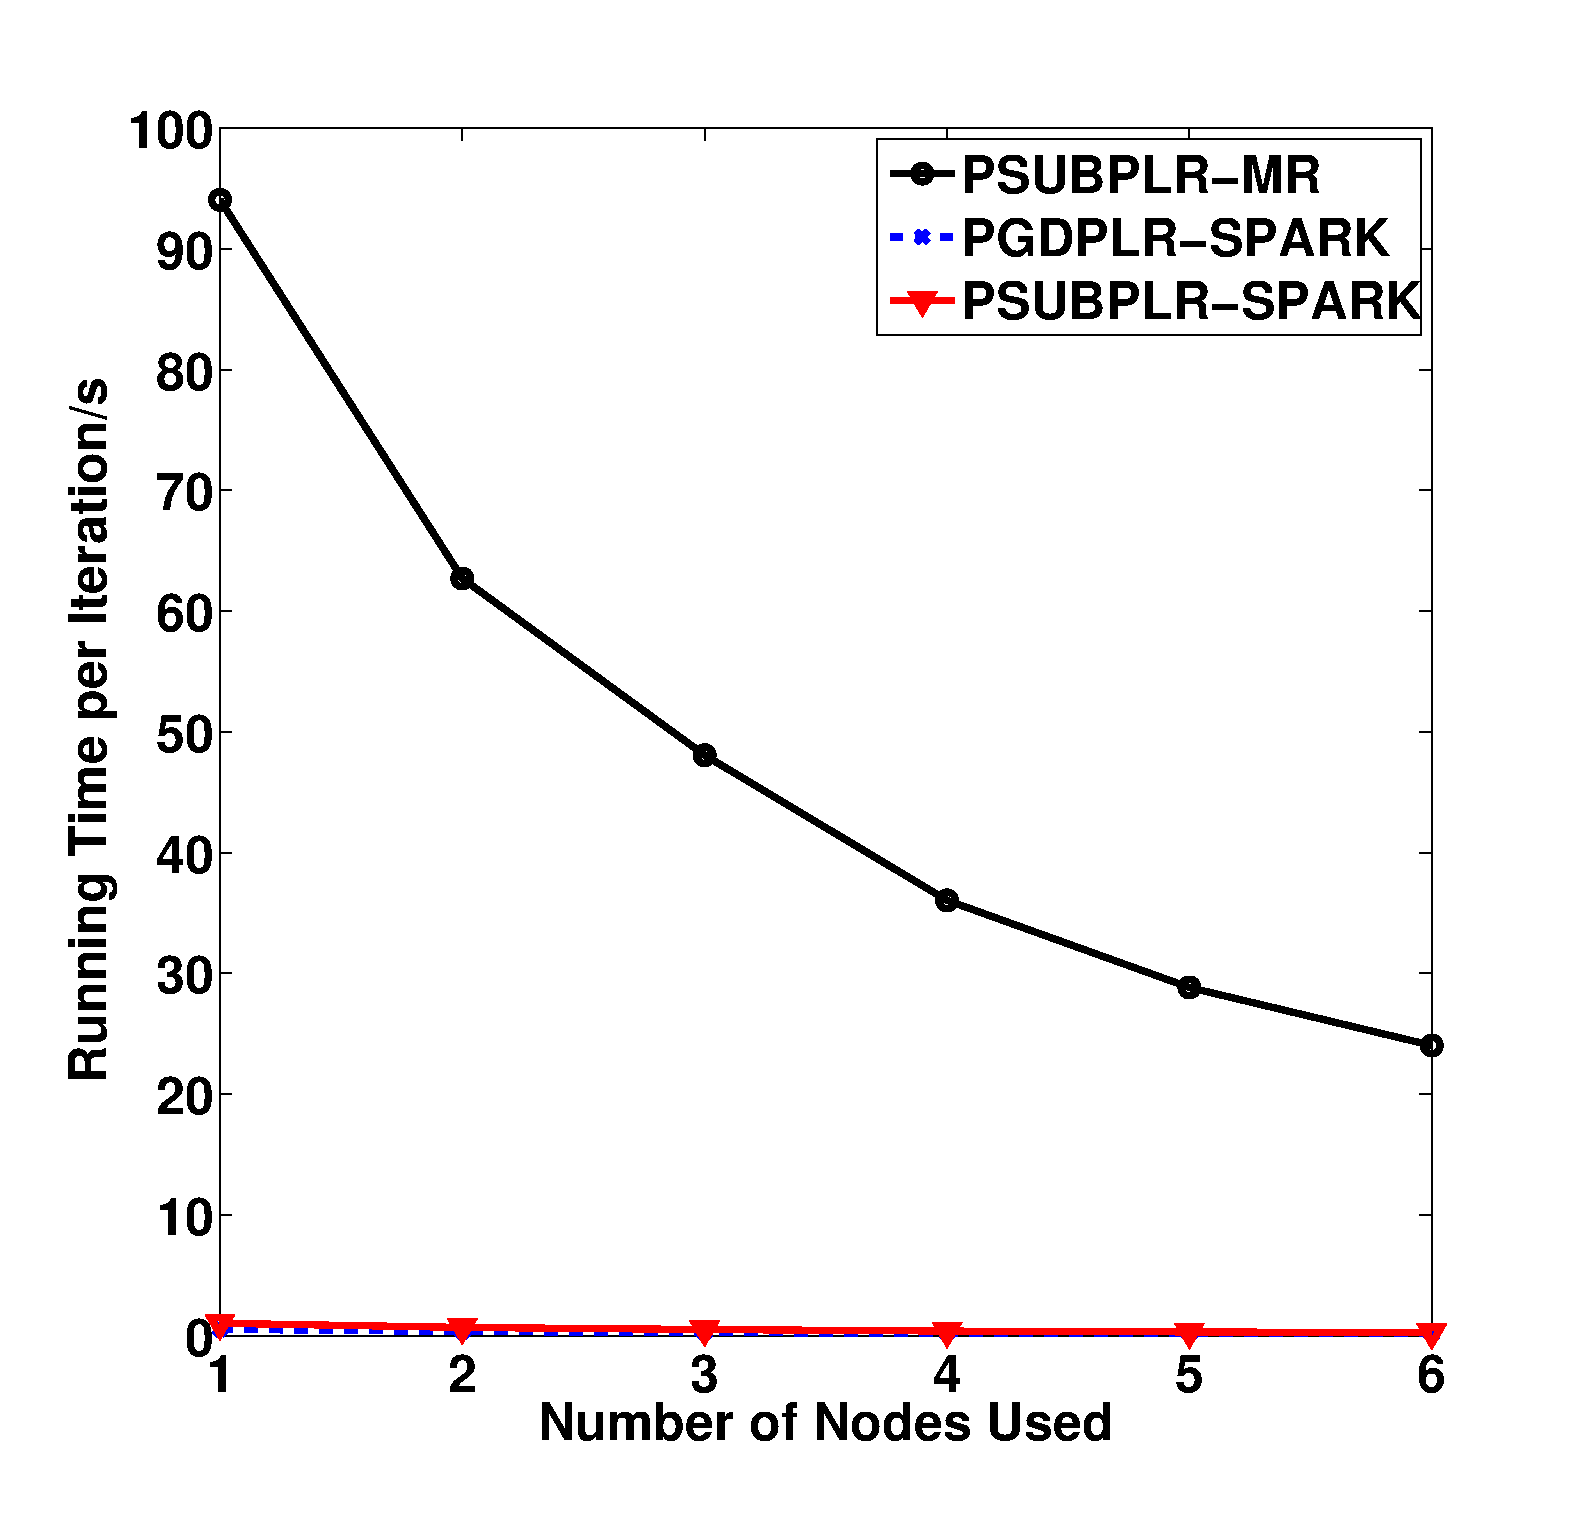
\includegraphics[height=4.5cm,width=5cm]{img/2d_time.eps}&
   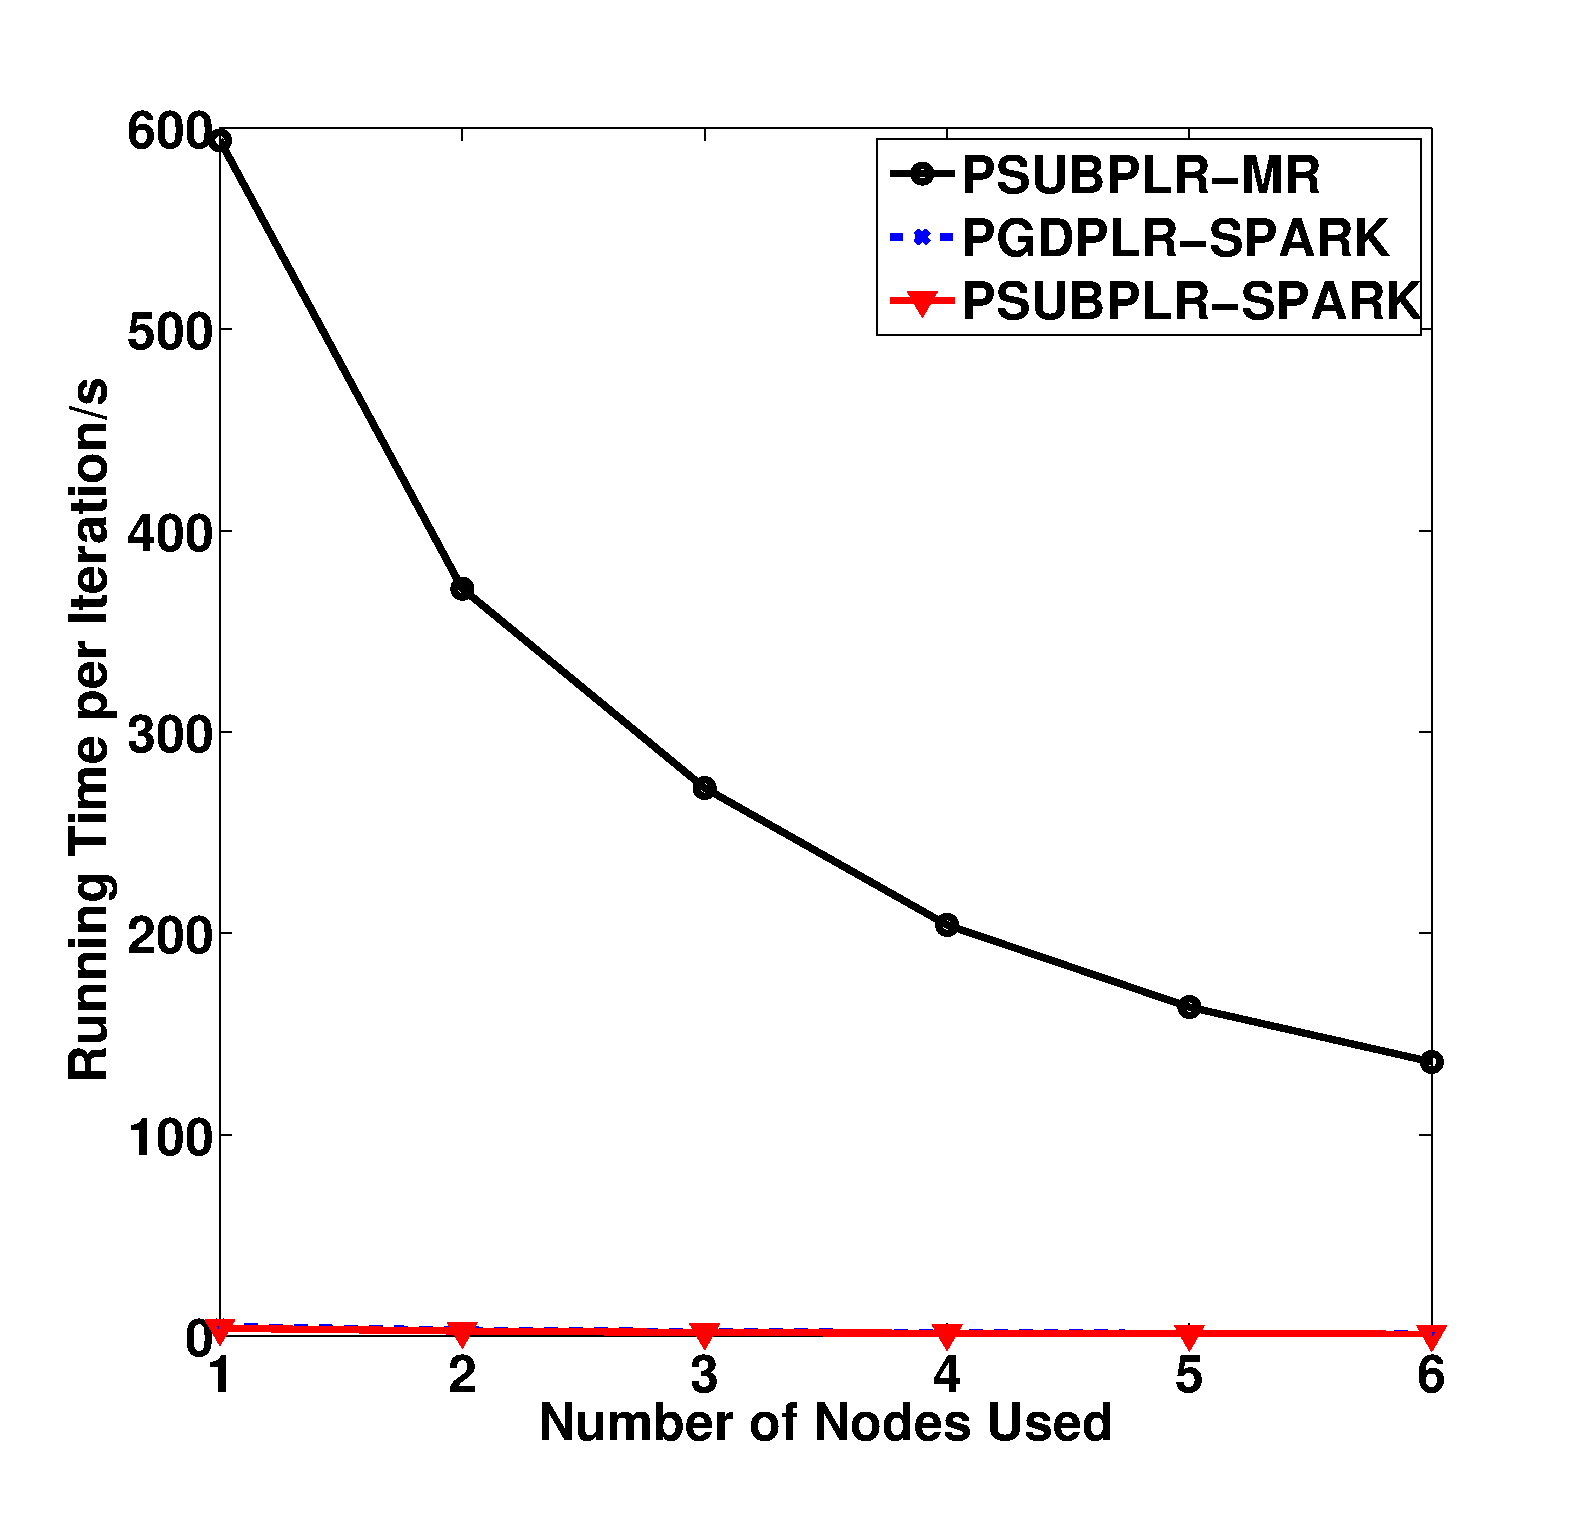
\includegraphics[height=3.9cm,width=4.5cm]{img/20NewsGroup_time.eps}&
   \hspace{-0.6cm}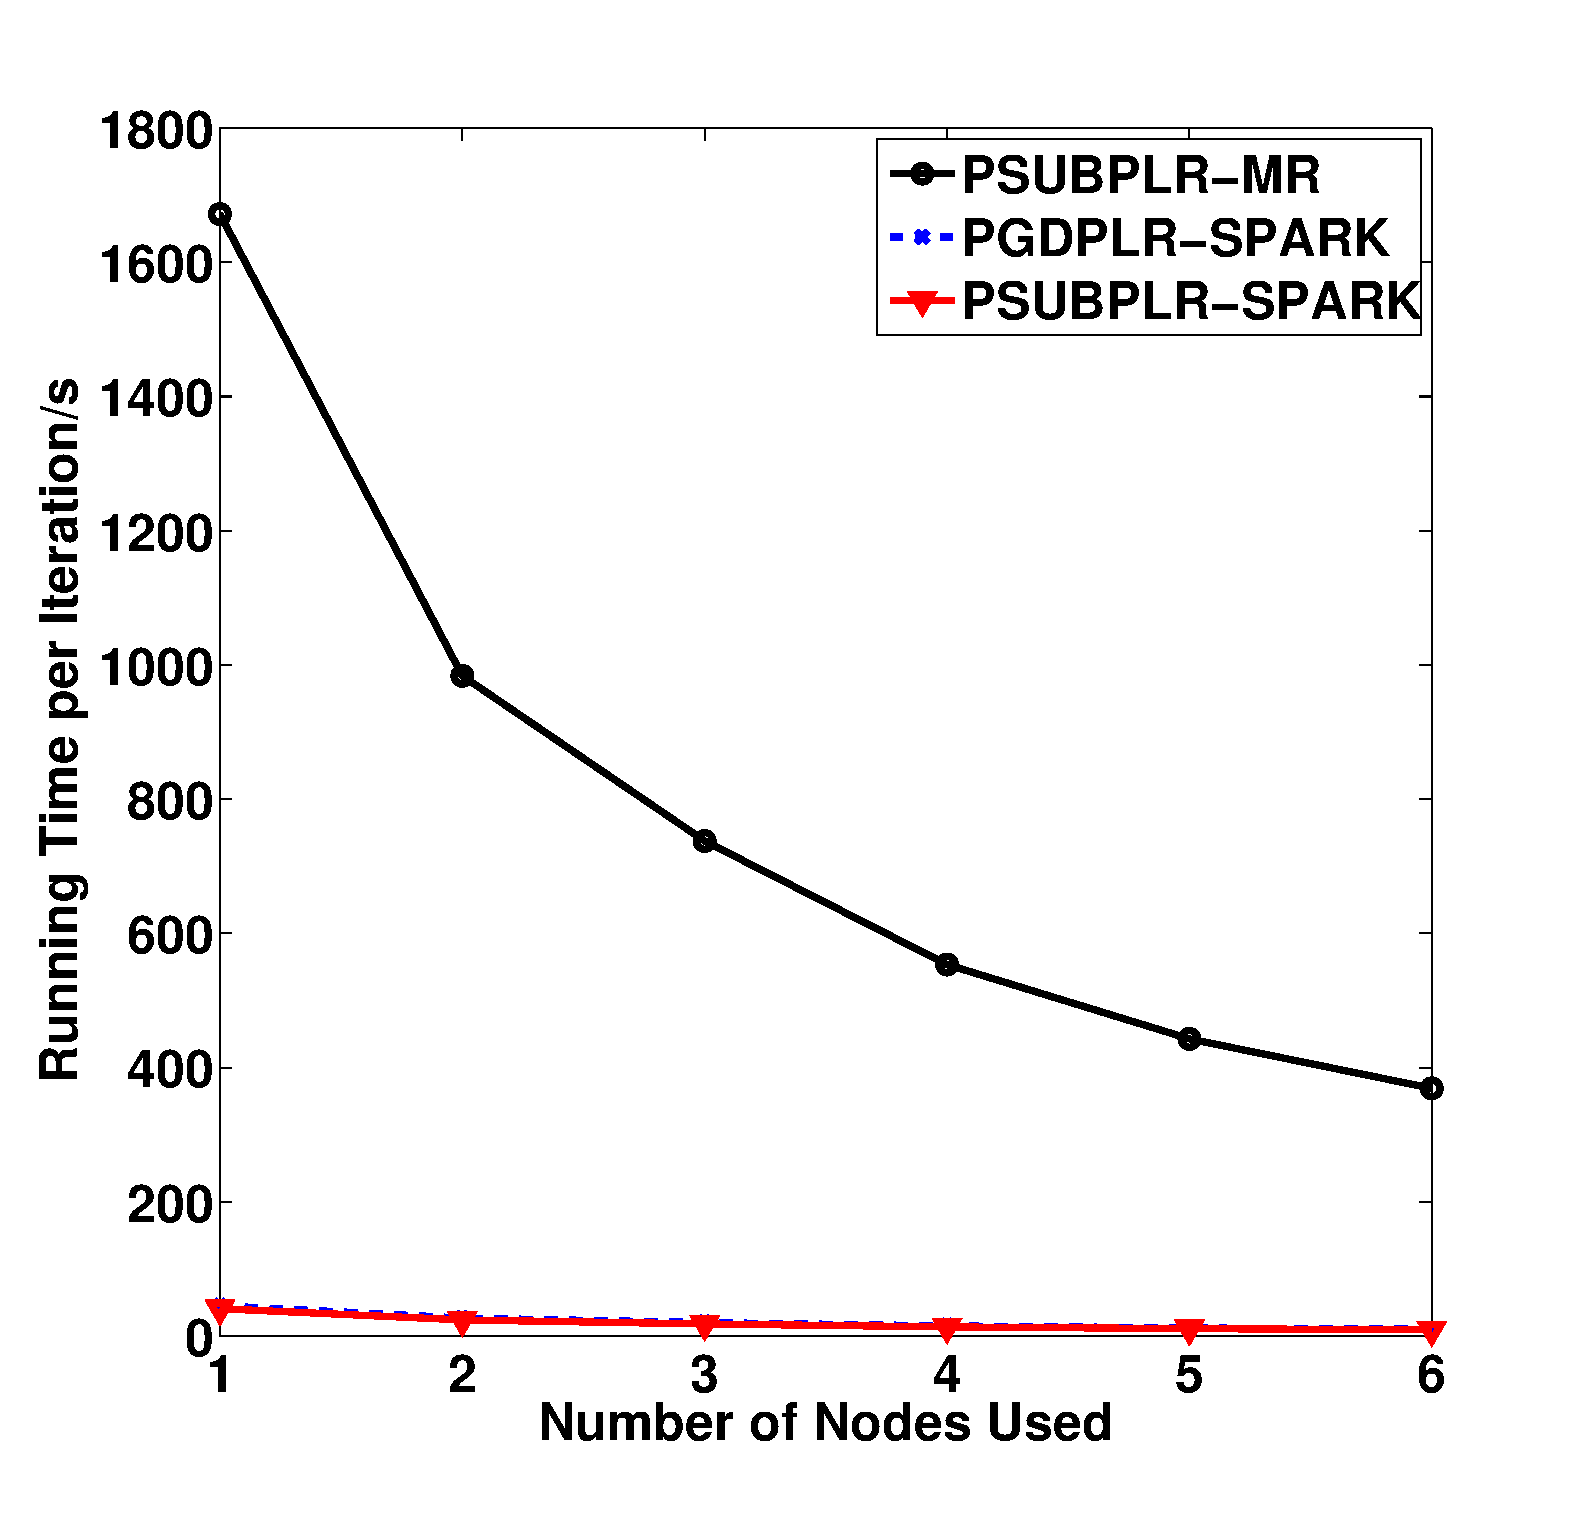
\includegraphics[height=3.9cm,width=4.5cm]{img/Gisette_time.eps}&
   \hspace{-0.6cm}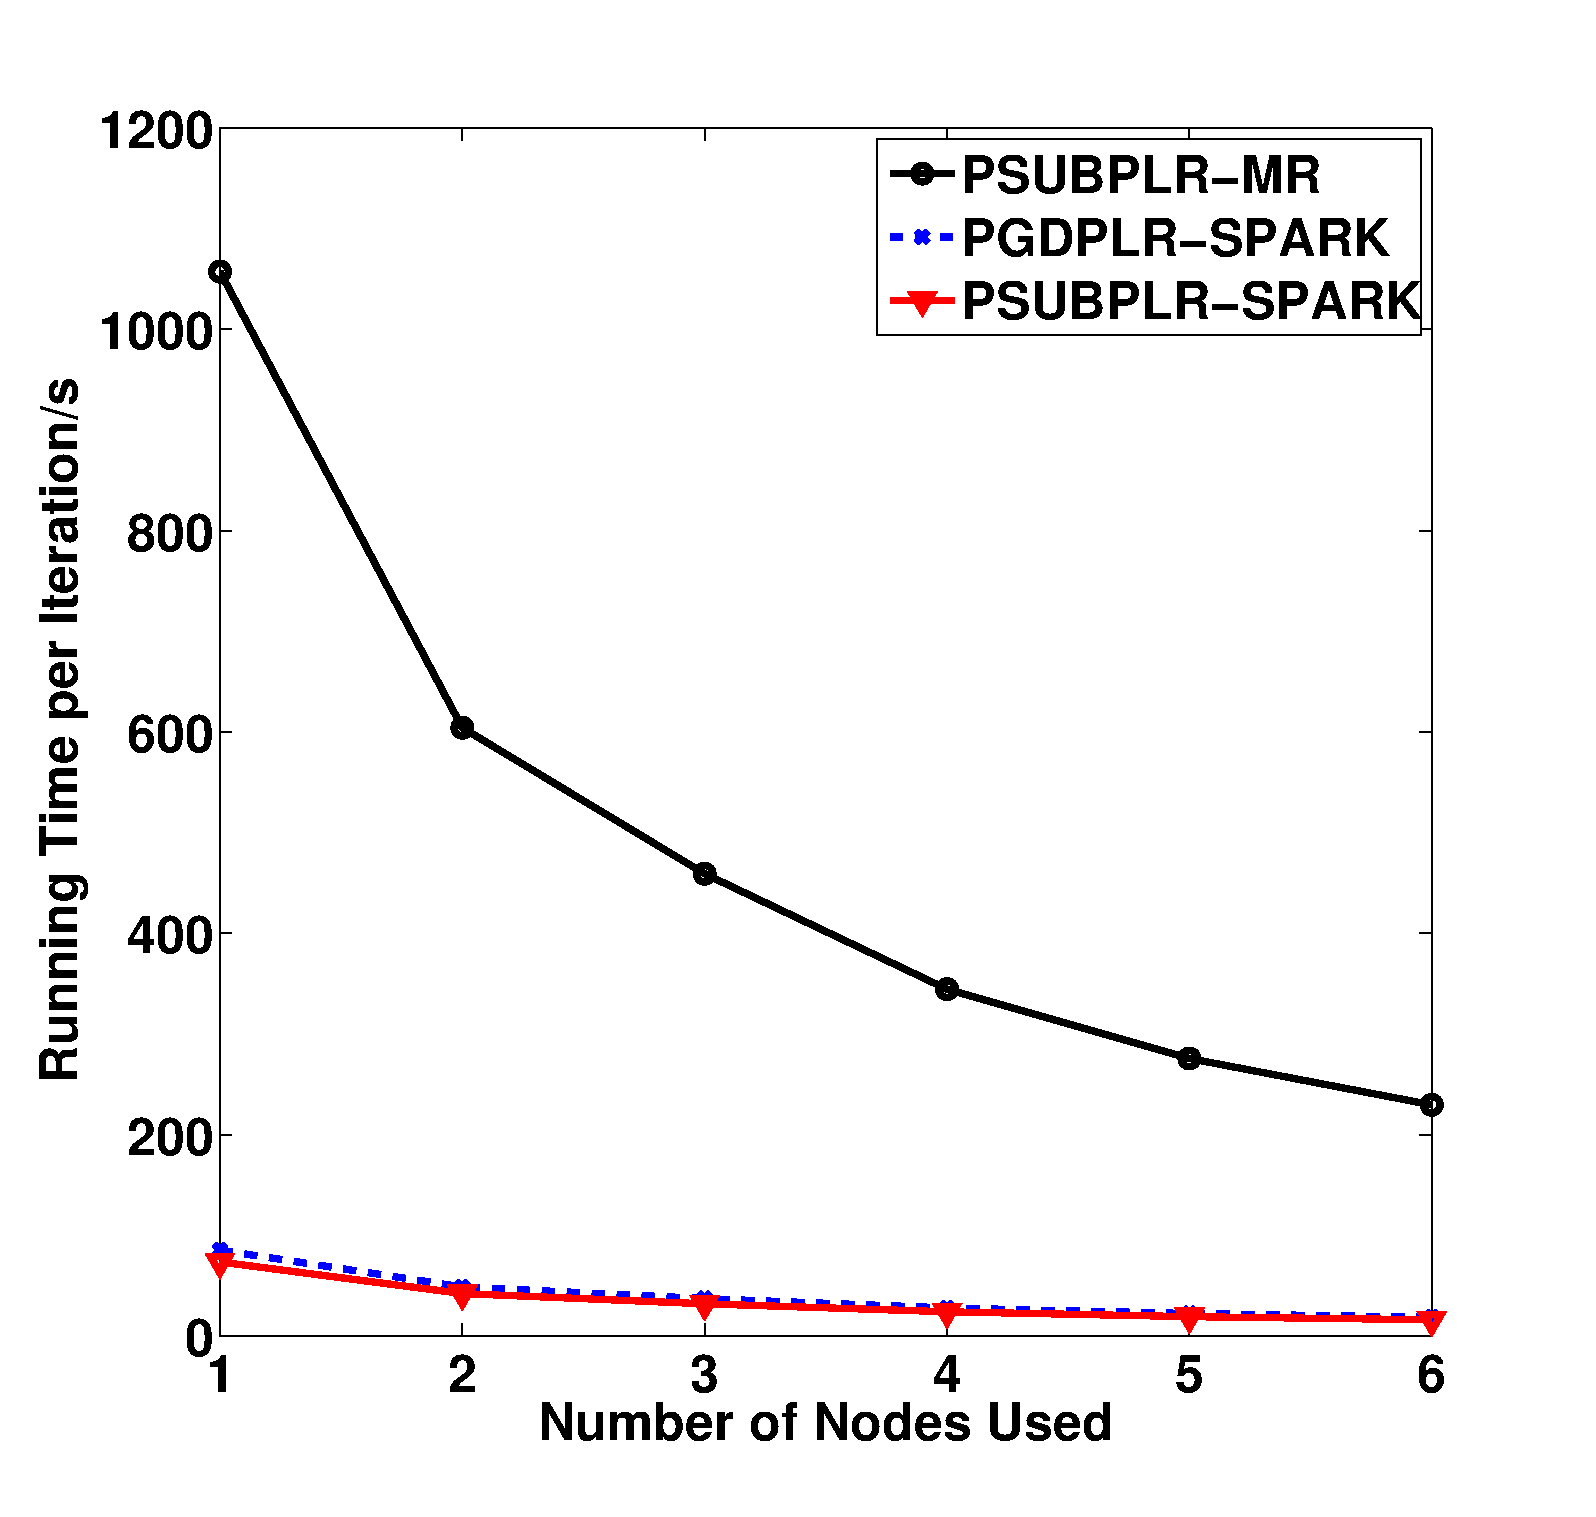
\includegraphics[height=3.9cm,width=4.5cm]{img/ECUESpam_time.eps}&
   \hspace{-0.6cm}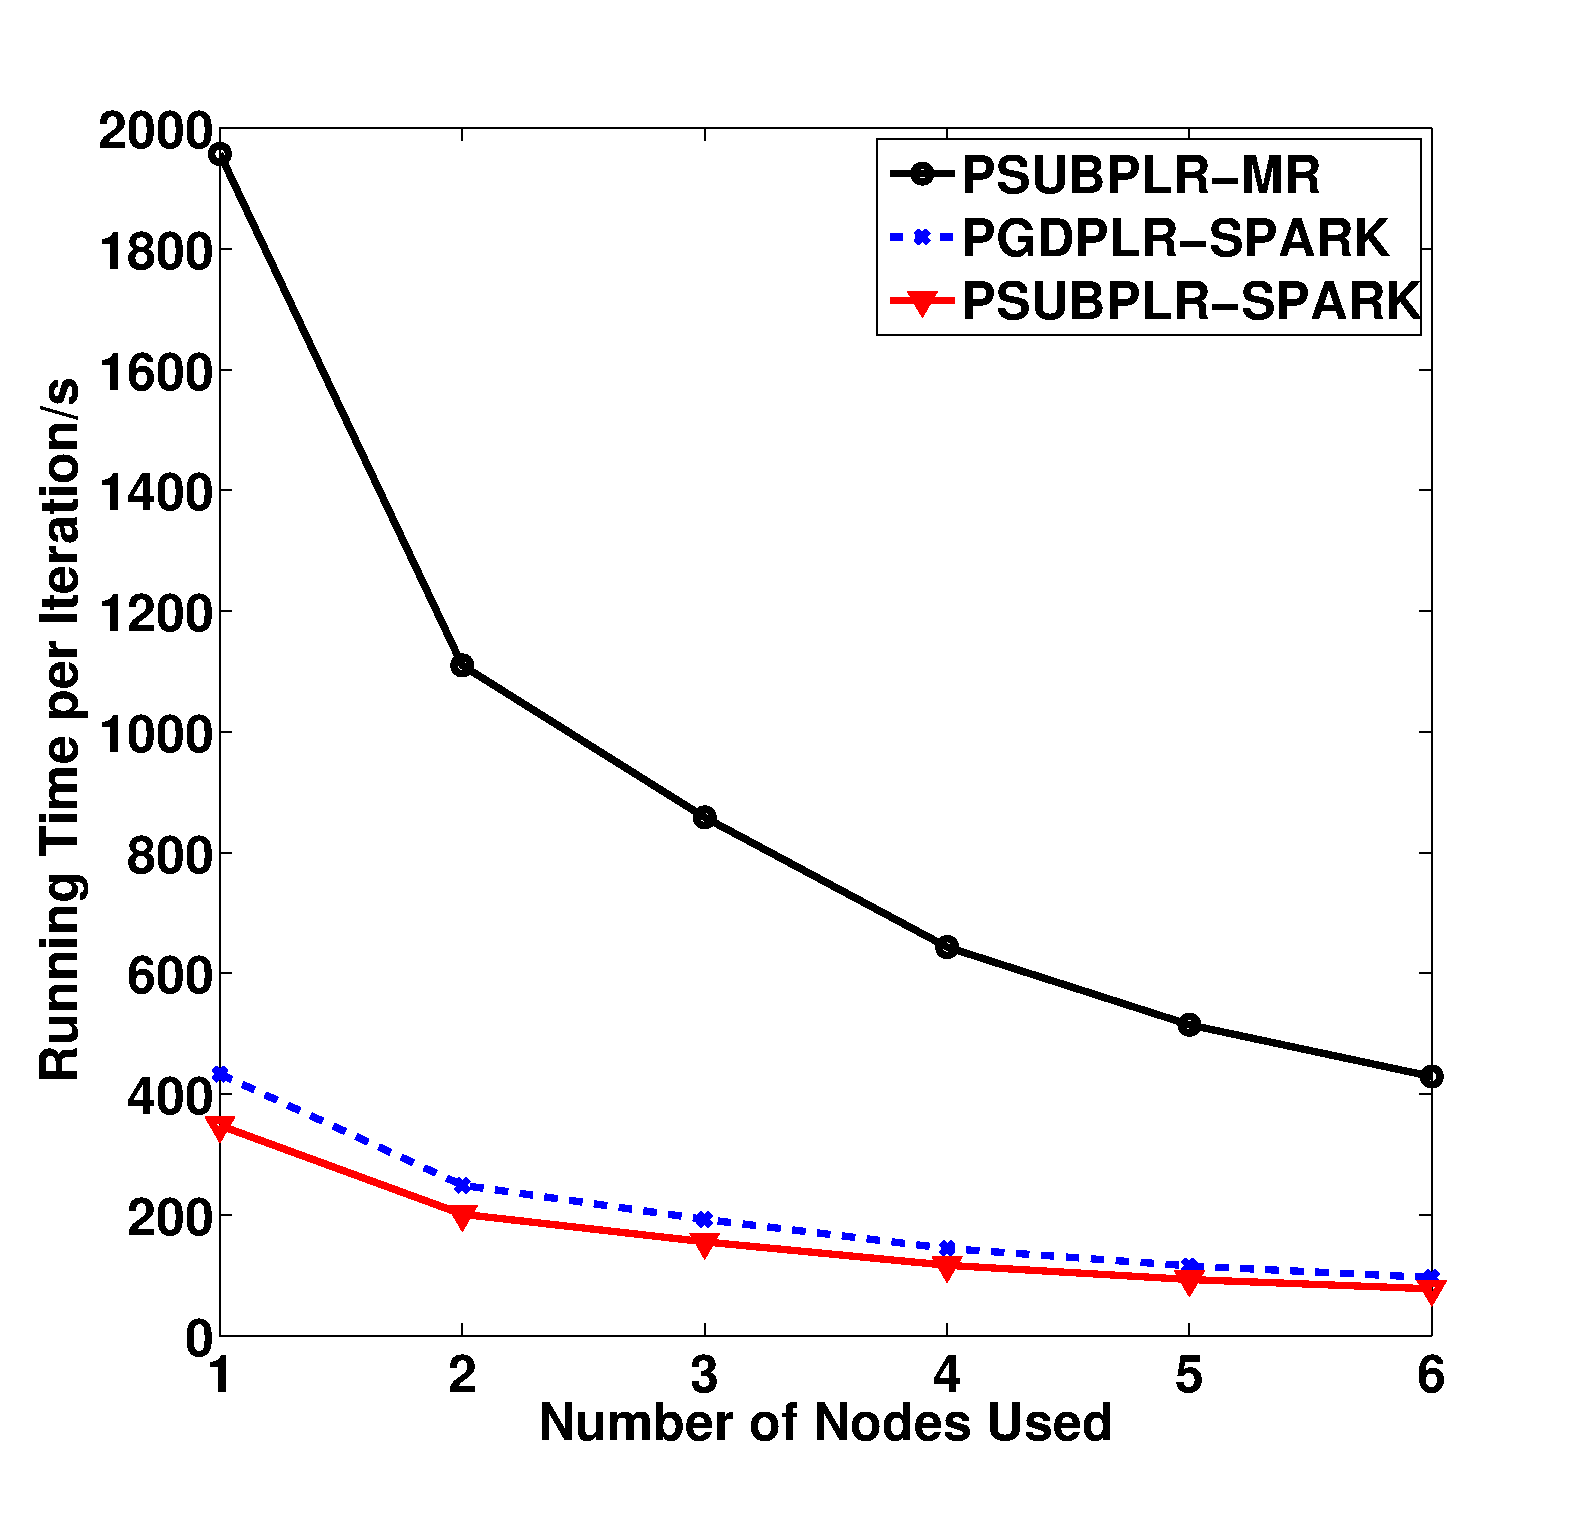
\includegraphics[height=3.9cm,width=4.5cm]{img/URL-Reputation_time.eps}\\
   (a) \textbf{20NewsGroup}. & \hspace{-0.3cm}(b) \textbf{Gisette}. & \hspace{-0.3cm}(c) \textbf{ECUESpam}. & \hspace{-0.3cm}(d) \textbf{URL-Reputation}.\\
   \end{tabular}
\end{center}\vspace{-0.3cm}
   \caption{Running time, as a function of used node number.}\vspace{-0.5cm}
\label{fig:time}
\end{figure*}
%
It is evident, as prior work (e.g., \cite{chang2011psvm}), has pointed out, that due to IO and communication overheads, the benefit of adding more nodes would eventually be wahed out.  Though we have only employed six nodes in this study, the figures already indicate speedup slows down when more nodes are used.  Therefore, to deal with big data, future work should pay more attention on reducing IO and communication overheads.

\subsection{Fault Tolerance}
There are both system level techniques and algorithm level techniques to provide fault tolerance in parallel computation.
Results are shown in Table~\ref{tab:table5}.
\begin{table}[h]
\centering
\caption{Fault Tolerance Analysis}\label{tab:table5}\vspace{-0.3cm}
\begin{tabular}{|c|c|c|}
\hline
           & System Level & Algorithm Level \\
\hline
PSUBPLR-MR & \Checkmark & \Checkmark \\
\hline
PGDPLR-SPARK & \Checkmark & \XSolid \\
\hline
PSUBPLR-SPARK & \Checkmark &  \Checkmark \\
\hline
\end{tabular}
\end{table}
Here, randomization is employed in all sublinear methods, thus providing algorithm level fault tolerance for PSUBPLR-MR and PSUBPLR-SPARK.
Hadoop and Spark can both provide system level fault tolerance, but in different ways. Hadoop employs HDFS, whereas Spark has RDDs.
Of all six test programs, PSUBPLR-MR and PSUBPLR-SPARK are fault-tolerant in both system level and algorithm level.

Fig.~\ref{fig:14} shows the iteration time as a function of percentage of failed maps on \textbf{URL-Reputation} dataset for all three parallel test programs running on six nodes.
The number of iterations of PSUBPLR-MR remains unaffected when {\em maps} fail.
Both PGDPLR-SPARK and PSUBPLR-SPARK increase number of iterations when {\em maps} fail,  because of RDD reconstruction. However, the increase is not significant.
In general, Hadoop spends more overhead than Spark to support fault tolerance, and hence Hadoop enjoys less impact during failure recovery.

\begin{figure}[tb]
\center 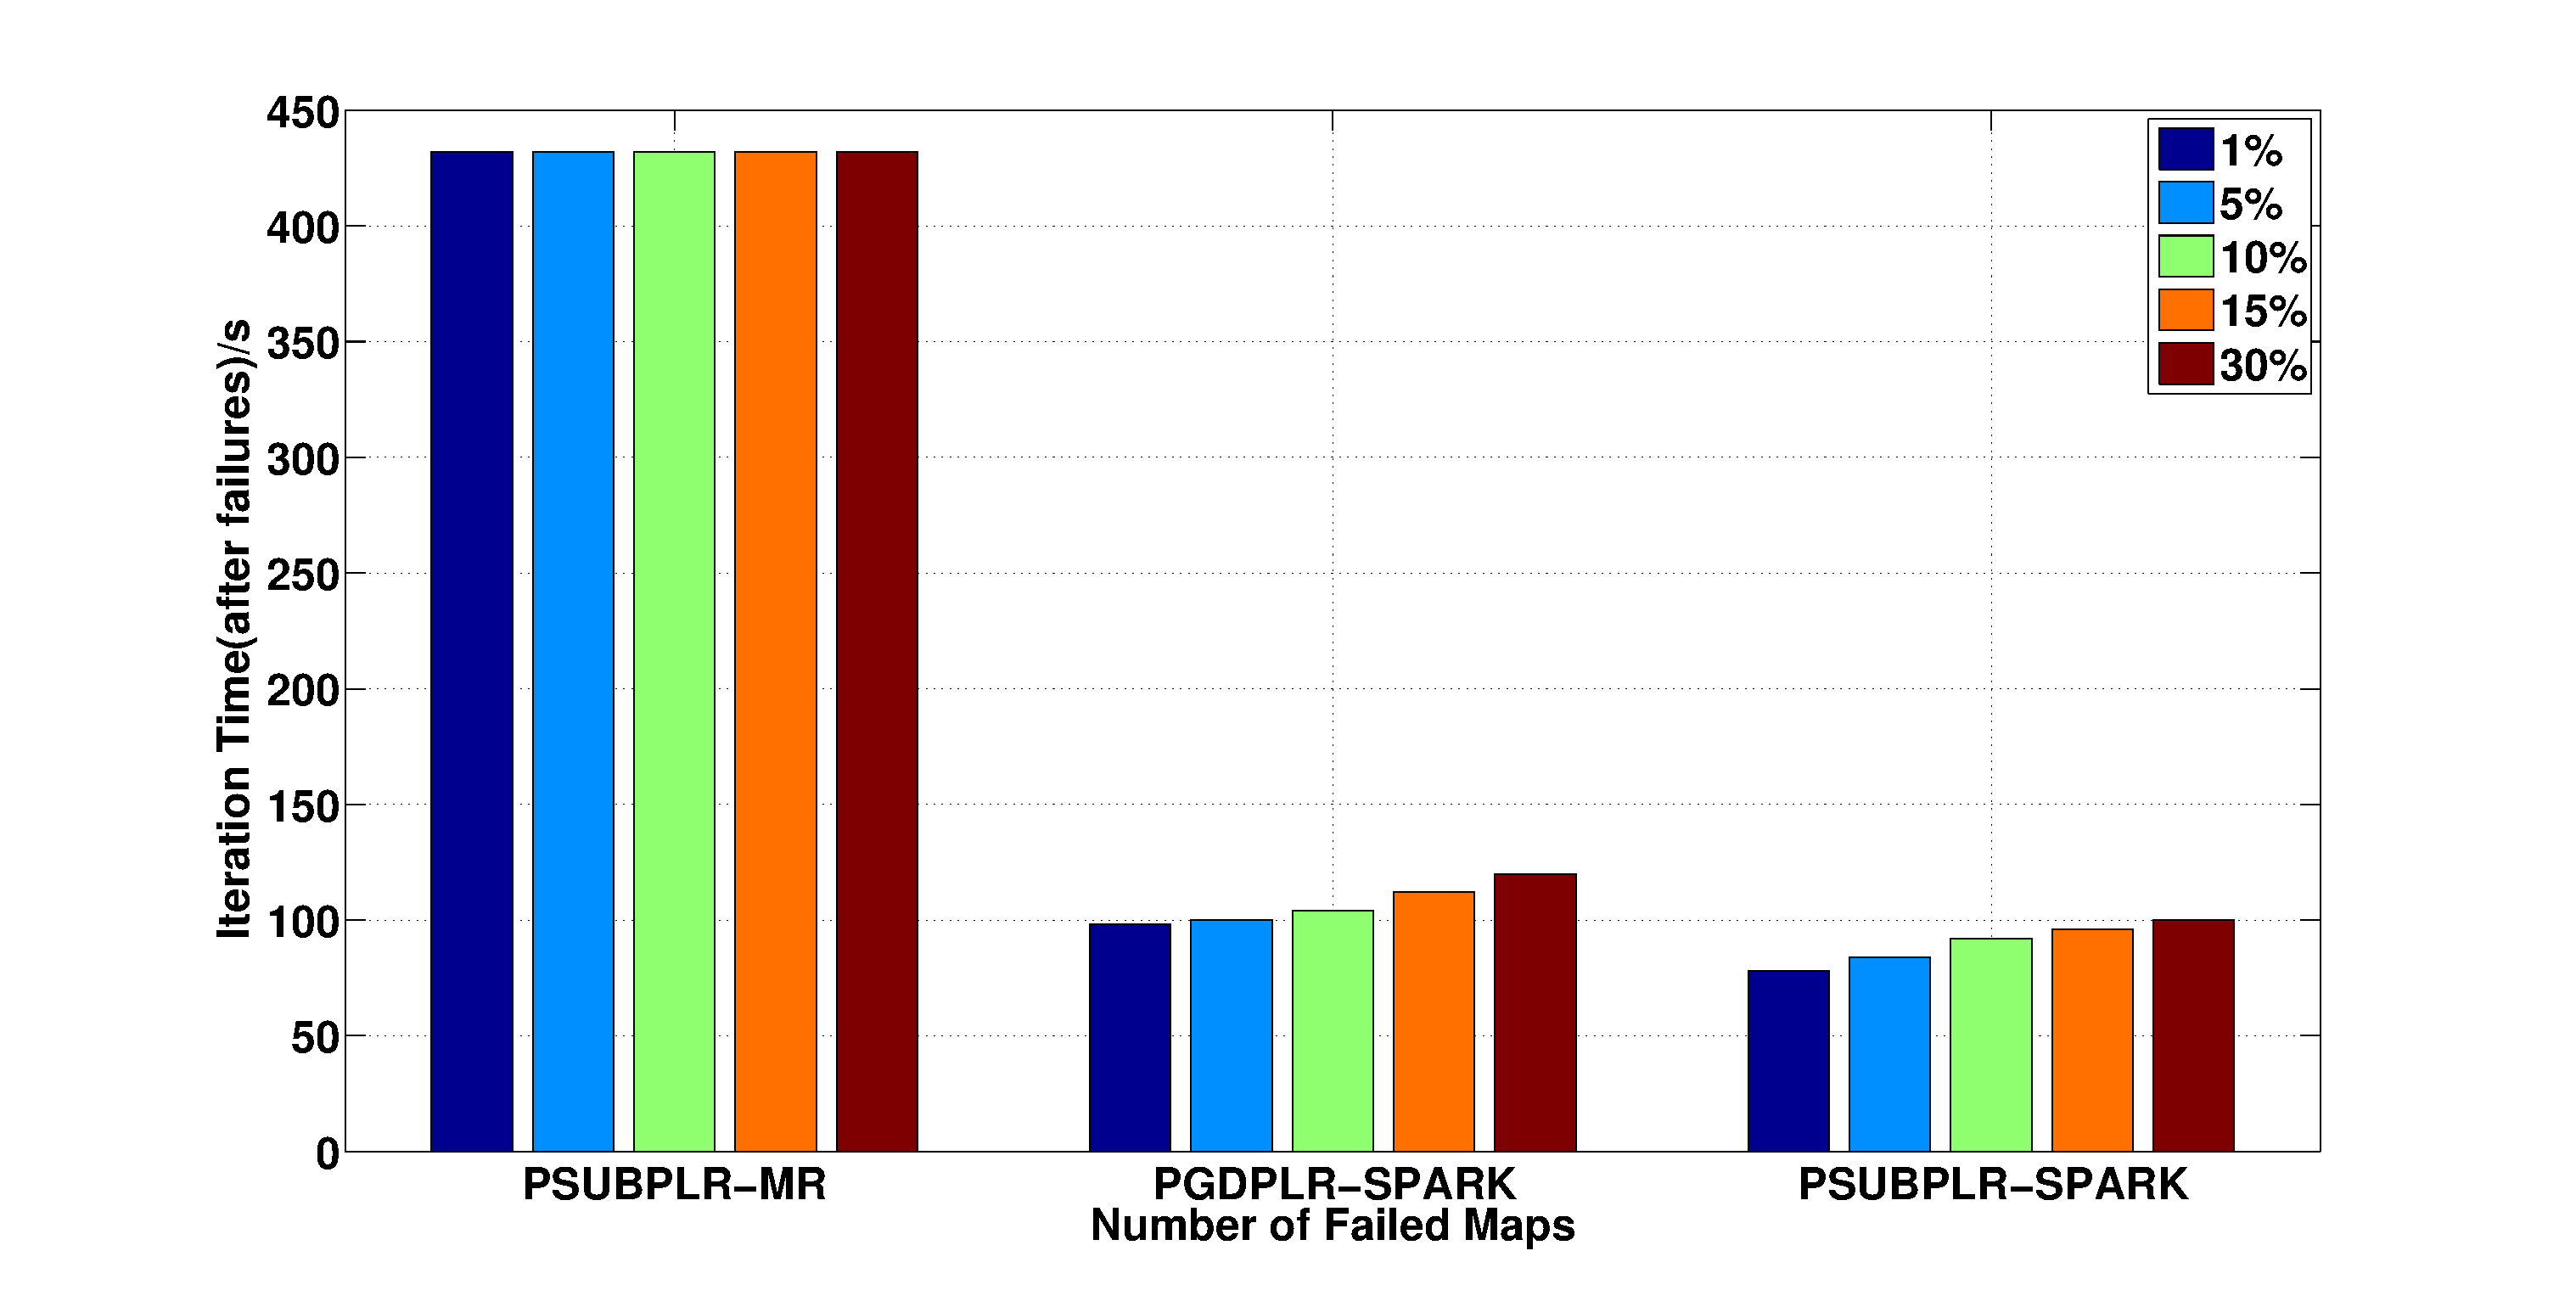
\includegraphics[height=4cm,width=8cm]{img/fault_tolerance.eps}\vspace{-0.3cm}
\caption{Iteration time, as a function of percentage of failed maps, on \textbf{URL-Reputation} Dataset, run on 6 nodes}\label{fig:14}\vspace{-0.5cm}
\end{figure}


\section{Conclusion} \label{sec:concl}
In this paper we analyzed three optimization approaches along with two computing platforms to train the LR model on large-scale, high-dimensional datasets for classification.  Based on extensive experiments, we summarized key features of each algorithm implemented on Hadoop and Spark.
We can conclude that sequential algorithms with memory intensive operations like Liblinear can perform very well if datasets can fit in memory.
For massive datasets, if limited by machine resources, Mahout with its online algorithm is a good choice with a slightly lower precision.
If machine resources are abundant, as Spark outperforms Hadoop for LR model training, we recommend choosing between parallel sublinear method and parallel gradient descent method (both on Spark) to trade off between speedup and precision.

Though we used only a six-node cluster to conduct experiments, our conclusions are expected to hold for larger datasets and more computing nodes.  We will validate this conjecture when we evaluate these algorithms in a production setting with a substantial larger cluster to deal with much larger application datasets.


\begin{small}
\bibliographystyle{plain}
\bibliography{mlpaper}
\end{small}
\end{document}
